% FORMAT AND PACKAGES
% {
\documentclass[a4paper]{article}
\usepackage{a4wide,amssymb,epsfig,latexsym,multicol,array,hhline,fancyhdr}
\usepackage{vntex}
\usepackage{verbatim}
\usepackage{amsmath}
\usepackage{lastpage}
\usepackage[lined,boxed,commentsnumbered]{algorithm2e}
\usepackage{enumerate}
\usepackage{xcolor}
\usepackage{graphicx}							% Standard graphics package
\usepackage{array}
\usepackage{tabularx, caption}
\usepackage{multirow}
\usepackage{multicol}
\usepackage{rotating}
\usepackage{graphics}
\usepackage{geometry}
\usepackage{listings}
\usepackage{setspace}
\usepackage{tabularx}
\usepackage{float}
\usepackage{epsfig}
\usepackage{tikz}
\usepackage{xfrac}
\usepackage{booktabs}
\usepackage{bm}
\usepackage[backend=bibtex,style=ieee]{biblatex}
\usepackage[colorlinks]{hyperref}
% \usepackage[acronym,toc]{glossaries}
% \usepackage[symbols,nogroupskip,nonumberlist]{glossaries-extra}
\usepackage[
 sort=none,% no sorting or indexing required
 abbreviations,% create list of abbreviations
 symbols,% create list of symbols
 stylemods,style=list, % set the default glossary style
 nogroupskip, nonumberlist, nomain
]{glossaries-extra}
\lstset{frame=tb,
  language=Python,
  aboveskip=3mm,
  belowskip=3mm,
  showstringspaces=false,
  columns=flexible,
  basicstyle={\small\ttfamily},
  numbers=none,
  numberstyle=\tiny\color{gray},
  keywordstyle=\color{blue},
  commentstyle=\color{dkgreen},
  stringstyle=\color{mauve},
  breaklines=true,
  breakatwhitespace=true,
  tabsize=3, 
  numbers=left, numberstyle=\tiny,
}

% FORMATTING
% {
\DeclareMathOperator{\arccot}{arccot}
\DeclareMathOperator*{\argmax}{arg\,max}
\DeclareMathOperator*{\argmin}{arg\,min}
\captionsetup[table]{name=Table}
\captionsetup[figure]{name=Figure}
\newenvironment{Description}{\list{}{%
    \let\makelabel\descriptionlabel    % this comes from the original description environment
    \setlength{\rightmargin}{\leftmargin}% this comes from the original quote environment
    \setlength{\labelwidth}{0pt}%          this is new
    }}{\endlist}

\addbibresource{citations.bib}
    
\hypersetup{urlcolor=blue,linkcolor=black,citecolor=black,colorlinks=true} 
\usetikzlibrary{arrows,snakes,backgrounds}
\definecolor{mathblue}{RGB}{0,114,188}
\definecolor{dkgreen}{rgb}{0,0.6,0}
\definecolor{mauve}{rgb}{0.58,0.0,0.83}

\newtheorem{theorem}{{\bf Theorem}}
\newtheorem{property}{{\bf Property}}
\newtheorem{proposition}{{\bf Proposition}}
\newtheorem{corollary}[proposition]{{\bf Corollary}}
\newtheorem{lemma}[proposition]{{\bf Lemma}}

\AtBeginDocument{\renewcommand*\contentsname{Mục lục}}
\AtBeginDocument{\renewcommand*\refname{Tài liệu tham khảo}}
%\usepackage{fancyhdr}

\setlength{\headheight}{40pt}
\pagestyle{fancy}
\fancyhead{} % clear all header fields
\fancyhead[L]{
 \begin{tabular}{rl}
    \begin{picture}(25,15)(0,0)
    \put(0,-8){
\includegraphics[width=8mm, height=8mm]{hcmut.png}}
    %\put(0,-8){
\epsfig{width=10mm,figure=hcmut.eps}}
   \end{picture}&
	%
\includegraphics[width=8mm, height=8mm]{hcmut.png} & %
	\begin{tabular}{l}
		\textbf{\bf \ttfamily Đại học Quốc gia TP.Hồ Chí Minh}\\
		\textbf{\bf \ttfamily Trường Đại học Bách Khoa}
	\end{tabular} 	
 \end{tabular}
}
\fancyhead[R]{
	\begin{tabular}{l}
		\tiny \bf \\
		\tiny \bf 
	\end{tabular}  }
\fancyfoot{} % clear all footer fields
\fancyfoot[L]{\scriptsize \ttfamily Báo cáo bài tập lớn - Xử lý ngôn ngữ tự nhiên (CO3086) - Năm học 2025-2026}
\fancyfoot[R]{\scriptsize \ttfamily Trang {\thepage}/\pageref{LastPage}}
\renewcommand{\headrulewidth}{0.3pt}
\renewcommand{\footrulewidth}{0.3pt}
\renewcommand{\figureautorefname}{hình}
\renewcommand{\tableautorefname}{bảng}
\captionsetup[figure]{name=Hình}
\captionsetup[table]{name=Bảng}
\setcounter{secnumdepth}{4}
\setcounter{tocdepth}{4}

\makeatletter
\newcounter {subsubsubsection}[subsubsection]
\renewcommand\thesubsubsubsection{\thesubsubsection .\@alph\c@subsubsubsection}
\newcommand\subsubsubsection{\@startsection{subsubsubsection}{4}{\z@}%
                                     {-3.25ex\@plus -1ex \@minus -.2ex}%
                                     {1.5ex \@plus .2ex}%
                                     {\normalfont\normalsize\bfseries}}
\newcommand*\l@subsubsubsection{\@dottedtocline{3}{10.0em}{4.1em}}
\newcommand*{\subsubsubsectionmark}[1]{}
\makeatother
\renewcommand{\subsectionautorefname}{mục}
% DOCUMENT
\begin{document}

% TITLE PAGE
\begin{titlepage}
\begin{center}
ĐẠI HỌC QUỐC GIA THÀNH PHỐ HỒ CHÍ MINH \\
TRƯỜNG ĐẠI HỌC BÁCH KHOA \\
KHOA KHOA HỌC VÀ KỸ THUẬT MÁY TÍNH
\end{center}

\vspace{1cm}

\begin{figure}[h!]
\begin{center}

\includegraphics[width=3cm]{hcmut.png}
\end{center}
\end{figure}

\vspace{1cm}

\begin{center}
\textbf{\LARGE BÁO CÁO BÀI TẬP LỚN} \\
\textbf{\LARGE XỬ LÝ NGÔN NGỮ TỰ NHIÊN (CO3086)} \\
\rule{8cm}{0.2mm} \\
\vspace{0.3cm}
\underline{\LARGE \textit{\textbf{ĐỀ TÀI:}}} \\
\vspace{0.4cm}
\LARGE \textbf{TRÍCH XUẤT THÔNG TIN VÀ PHÂN TÍCH NGỮ NGHĨA HỢP ĐỒNG PHÁP LÝ} \\
\vspace{0.5cm}
{\fontsize{14pt}{14pt}\selectfont GV hướng dẫn: Bùi Văn Quốc Bảo} \\
\vspace{0.5cm}
{\fontsize{14pt}{14pt}\selectfont Sinh viên thực hiện: Nguyễn Văn Đức - 2310790} \\
{\fontsize{14pt}{14pt}\selectfont Lớp: L02} \\
\vspace{0.3cm}


\end{center}
\vspace{1.3cm}
\begin{center}
{TP. HỒ CHÍ MINH, 04/2026 }
\end{center}

\end{titlepage}

\pagebreak
\tableofcontents
\pagebreak

\section{Tổng quan đề tài}

\subsection{Đặt vấn đề}
Trong bối cảnh số hóa và tự động hóa quy trình doanh nghiệp ngày càng phát triển, việc xử lý và quản lý khối lượng lớn các văn bản pháp lý, đặc biệt là hợp đồng, trở thành một bài toán đầy thách thức. Các hợp đồng pháp lý tiếng Việt thường chứa những câu văn dài, cấu trúc ngữ pháp phức tạp, nhiều mệnh đề phụ, điều kiện và các phép liệt kê đan xen. Việc đọc hiểu, trích xuất thông tin và phân tích rủi ro thủ công không chỉ tiêu tốn nhiều thời gian, nguồn lực mà còn tiềm ẩn nguy cơ sai sót cao do yếu tố chủ quan của con người. 

Do đó, nhu cầu cấp thiết đặt ra là phải xây dựng các hệ thống tự động có khả năng "hiểu" ngôn ngữ pháp lý thô (unstructured text), trích xuất được các thông tin cốt lõi (như chủ thể tham gia, số tiền, thời hạn) và phân tích được ngữ nghĩa của từng điều khoản (điều kiện phạt là gì, quyền và nghĩa vụ của các bên ra sao). Việc ứng dụng Xử lý Ngôn ngữ Tự nhiên (NLP) vào miền dữ liệu pháp lý chính là giải pháp tối ưu nhằm chuyển đổi dữ liệu văn bản thô thành các cấu trúc tri thức có ý nghĩa, phục vụ cho việc tự động hóa tra cứu và quản trị rủi ro.

\subsection{Mục tiêu đề tài}
Mục tiêu chính của đề tài là nghiên cứu, thiết kế và triển khai một NLP pipeline toàn diện để phân tích các hợp đồng pháp lý tiếng Việt. Dự án được cấu trúc thành ba mục tiêu cụ thể như sau:

\begin{itemize}
    \item \textbf{Tiền xử lý và Phân tích cú pháp (Assignment 1):} Xây dựng công cụ phân tách các câu phức tạp thành các mệnh đề độc lập về mặt ngữ nghĩa (Clause Segmentation); gắn nhãn và phân rã cụm danh từ (Noun Phrase Chunking) theo lược đồ IOB; thực hiện phân tích cú pháp phụ thuộc (Dependency Parsing) để làm rõ mối quan hệ chủ - vị ngữ và các thành phần bổ nghĩa trong câu.
    \item \textbf{Trích xuất thông tin và Phân tích ngữ nghĩa (Assignment 2):} Xây dựng và tinh chỉnh (fine-tune) mô hình Nhận dạng thực thể có tên (NER) chuyên biệt cho lĩnh vực hợp đồng (nhận diện PARTY, MONEY, DATE, RATE, PENALTY, LAW); triển khai Gắn nhãn vai trò ngữ nghĩa (Semantic Role Labeling - SRL) để trả lời cho câu hỏi "ai làm gì với ai, trong điều kiện nào"; và Phân loại ý định mệnh đề (Intent Classification) nhằm xác định chức năng pháp lý của điều khoản (Obligation, Right, Prohibition, Termination Condition).
    \item \textbf{Ứng dụng hỏi đáp hợp đồng (Assignment 3):} Xây dựng một hệ thống Chatbot Hỏi đáp thông minh dựa trên kỹ thuật Retrieval-Augmented Generation - RAG. Hệ thống cho phép người dùng truy vấn thông tin hợp đồng bằng ngôn ngữ tự nhiên, kết hợp dữ liệu vector ngữ nghĩa và metadata cấu trúc (NER, SRL, Intent) để đưa ra câu trả lời chính xác, tránh hiện tượng "ảo giác" (hallucination) và cung cấp nguồn trích dẫn rõ ràng.
\end{itemize}

\subsection{Phạm vi đề tài}
\begin{itemize}
    \item \textbf{Dữ liệu:} Đề tài tập trung xử lý các loại hợp đồng pháp lý thông dụng tại Việt Nam (như hợp đồng mua bán, hợp đồng thuê nhà, hợp đồng lao động, hợp đồng dịch vụ, v.v.). Dữ liệu thô ban đầu (PDF, DOCX) được thu thập, sau đó sử dụng LLM (Gemini) để chuyển sang dạng văn bản thuần túy (TXT) đã được làm sạch và thêm metadata cần thiết.
    \item \textbf{Kỹ thuật và Mô hình NLP:} Kết hợp linh hoạt giữa các quy tắc (Rule-based), công cụ NLP mã nguồn mở (Underthesea) cho các tác vụ cơ sở, và các mô hình Học sâu (Deep Learning) dựa trên kiến trúc Transformer. Cụ thể, dự án tiến hành fine-tune mô hình \textit{PhoBERT} cho hầu hết các tác vụ như tách câu, NER, SRL và Intent Classification.
    \item \textbf{Kiến trúc hệ thống RAG:} Tích hợp cơ sở dữ liệu vector \textit{ChromaDB} để lưu trữ và truy xuất các mệnh đề, sử dụng mô hình embedding đa ngữ, và tận dụng API của \textit{Google Gemini} đóng vai trò LLM để sinh câu trả lời trong pipeline của \textit{LangChain}. Giao diện người dùng (UI) được triển khai trên nền tảng \textit{Streamlit}.
\end{itemize}
\pagebreak
\section{Cơ sở lý thuyết và công cụ}

\subsection{Cơ sở lý thuyết}

\subsubsection{Các bài toán NLP cơ bản}
\begin{itemize}
\item \textbf{Tách câu và mệnh đề (Clause Segmentation):}
Trong văn bản pháp lý, các điều khoản thường chứa câu phức với nhiều mệnh đề phụ hoặc danh sách liệt kê. Việc phân tách câu (segmentation) nhằm chia nhỏ văn bản thành các đơn vị ý nghĩa độc lập, tạo tiền đề cho các bước phân tích sau. Trong đồ án này, bài toán tách câu được mô hình hóa dưới dạng bài toán gán nhãn chuỗi (Sequence Labeling), xác định ranh giới mệnh đề kết hợp với xử lý luật (Rule-based) để tái tạo lại câu hoàn chỉnh.
\item \textbf{Phân cụm danh từ (Noun Phrase Chunking):}
Phân cụm danh từ là quá trình nhóm các từ liền kề nhau thành một cụm từ có chức năng như một danh từ trong câu. Quá trình này thường sử dụng lược đồ gán nhãn BIO (Begin - Inside - Outside) hoặc IOB2. Cụ thể, 'B-NP' đánh dấu từ bắt đầu cụm, 'I-NP' đánh dấu các từ bên trong cụm, và 'O' đánh dấu các từ nằm ngoài cụm.
\item \textbf{Phân tích cú pháp phụ thuộc (Dependency Parsing):}
Phân tích phụ thuộc là việc xác định các mối quan hệ ngữ pháp giữa các từ trong một câu. Cấu trúc này được biểu diễn dưới dạng một cây có hướng, trong đó một từ đóng vai trò là từ trung tâm (head) và các từ khác là phụ thuộc (dependent) với một nhãn quan hệ cụ thể (ví dụ: \textit{nsubj} - chủ ngữ, \textit{obj} - tân ngữ, \textit{root} - động từ chính).
\end{itemize}

\subsubsection{Trích xuất Thông tin và Ngữ nghĩa}
\begin{itemize}
\item \textbf{Nhận dạng thực thể có tên (Named Entity Recognition - NER):}
NER là tác vụ trích xuất và phân loại các cụm từ quan trọng trong văn bản vào các danh mục định trước. Đối với miền pháp lý, lược đồ thực thể tùy chỉnh thường phức tạp hơn, bao gồm: \textit{PARTY} (Chủ thể), \textit{MONEY} (Số tiền), \textit{DATE} (Thời gian), \textit{PENALTY} (Điều khoản phạt), \textit{LAW} (Luật áp dụng)... Mô hình NER thường được giải quyết bằng các kiến trúc học sâu như BiLSTM-CRF hoặc các mô hình ngôn ngữ lớn dựa trên Transformer.

\item \textbf{Gán nhãn vai trò ngữ nghĩa (Semantic Role Labeling - SRL):}
SRL nhằm mục đích trả lời câu hỏi "Ai làm gì cho ai, ở đâu, khi nào, và như thế nào?" đối với mỗi vị ngữ (predicate) trong câu. Các vai trò ngữ nghĩa (Arguments) thường bao gồm: \textit{Agent} (tác nhân gây ra hành động), \textit{Theme} (đối tượng chịu tác động), \textit{Recipient} (người nhận), và \textit{Time/Location} (thời gian/địa điểm). Trong bài tập lớn này, SRL kết hợp đặc trưng từ NER và Dependency Parsing để tăng cường độ chính xác.

\item \textbf{Phân loại ý định (Intent Classification):}
Đây là bài toán phân loại câu (Text Classification) nhằm gán nhãn chức năng pháp lý cho một điều khoản. Các nhãn thường bao gồm: \textit{Obligation} (Nghĩa vụ), \textit{Prohibition} (Điều cấm), \textit{Right} (Quyền lợi) và \textit{Termination Condition} (Điều kiện chấm dứt). Bài toán có thể giải quyết bằng các phương pháp Machine Learning truyền thống (TF-IDF kết hợp Logistic Regression) hoặc tinh chỉnh (fine-tune) các mô hình Transformer.
\end{itemize}


\subsubsection{Mô hình ngôn ngữ Transformer và PhoBERT}
\begin{itemize}
\item \textbf{Kiến trúc Transformer:}
Khác với RNN/LSTM truyền thống xử lý dữ liệu tuần tự, Transformer sử dụng cơ chế tự chú ý (Self-Attention) cho phép mô hình nhìn vào toàn bộ ngữ cảnh của câu cùng một lúc, giải quyết triệt để vấn đề phụ thuộc xa (long-term dependency) và cho phép huấn luyện song song \autocite{vaswani}.

\item \textbf{PhoBERT:}
PhoBERT \autocite{phobert} là mô hình ngôn ngữ tiền huấn luyện (Pre-trained Language Model) dựa trên kiến trúc RoBERTa, được huấn luyện đặc biệt cho tiếng Việt với kho dữ liệu khổng lồ (20GB văn bản thô). Việc fine-tune PhoBERT mang lại hiệu quả vượt trội cho các tác vụ hiểu ngôn ngữ tự nhiên tiếng Việt như NER, SRL và Text Classification. Trong dự án, để chống lại nhiễu dữ liệu và giảm overfitting, kỹ thuật \textit{Multi-Sample Dropout} \autocite{multidrop} được tích hợp vào kiến trúc phân loại của PhoBERT.
\end{itemize}


\subsubsection{Hệ thống Hỏi đáp kết hợp Truy xuất (Retrieval-Augmented Generation - RAG)}

RAG là một kiến trúc kết hợp giữa khả năng truy xuất thông tin truyền thống (Information Retrieval) và khả năng sinh văn bản của Mô hình Ngôn ngữ Lớn (LLM). Thay vì dựa hoàn toàn vào tham số nội tại, RAG truy xuất các tài liệu/mệnh đề có liên quan nhất từ một Cơ sở dữ liệu Vector (Vector Database) dựa trên câu hỏi của người dùng. Các tài liệu này sau đó được ghép vào ngữ cảnh (context prompt) để LLM sinh ra câu trả lời chính xác, có cơ sở và giảm thiểu tối đa hiện tượng "ảo giác" (hallucination) \autocite{retrieval}.

% [Placeholder: Hình minh họa kiến trúc RAG]
\begin{figure}[H]
    \centering
    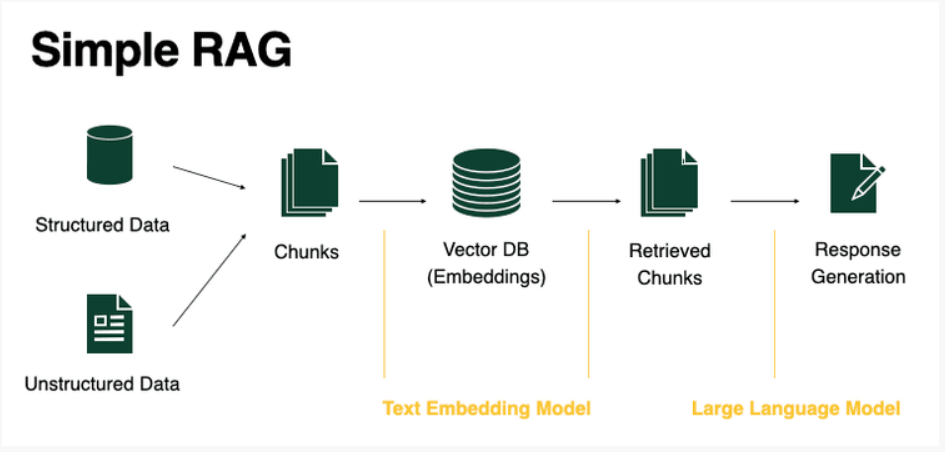
\includegraphics[width=1.0\textwidth]{Image/simple_rag.png}
    \caption{Kiến trúc tổng quan của hệ thống RAG. Nguồn: \href{https://www.bentoml.com/blog/building-rag-with-open-source-and-custom-ai-models}{Simple RAG}.}
    \label{fig:rag_arch}
\end{figure}

\subsection{Công cụ và thư viện}
Để triển khai hệ thống, đồ án sử dụng các công cụ và thư viện mã nguồn mở sau:
\begin{itemize}
    \item \textbf{Stanza \& Underthesea:} Các bộ công cụ NLP chuyên dụng. Underthesea được sử dụng để tách từ tiếng Việt (Word Segmentation), trong khi Stanza (phát triển bởi Stanford NLP) được cấu hình offline để phân tích cú pháp phụ thuộc (Dependency Parsing) và gán nhãn từ loại với độ chính xác cao.
    \item \textbf{HuggingFace Transformers \& PyTorch:} Nền tảng cốt lõi để tải, tinh chỉnh (fine-tune) và thực hiện suy diễn (inference) mô hình PhoBERT. Khung PyTorch cho phép tùy biến sâu các hàm mất mát (như \textit{Focal Loss}) và kiến trúc mạng học sâu bổ sung (như \textit{BiLSTM} cho tác vụ SRL).
    \item \textbf{ChromaDB:} Cơ sở dữ liệu Vector mã nguồn mở, được tích hợp qua LangChain, giúp lưu trữ embedding của các mệnh đề hợp đồng và siêu dữ liệu (metadata) hỗ trợ truy vấn lọc ngữ nghĩa tốc độ cao.
    \item \textbf{Google GenAI (Gemini 3.1 Flash):} API mô hình ngôn ngữ lớn đóng vai trò là khối sinh (Generator) trong pipeline RAG, cũng như góp phần hỗ trợ làm sạch/chuyển đổi văn bản hợp đồng thô ở khâu tiền xử lý một cách tự động.
    \item \textbf{FastAPI \& Streamlit:} FastAPI được dùng để xây dựng các API xử lý ngôn ngữ chịu tải cao, cung cấp backend kết nối với mô hình AI. Streamlit được dùng để xây dựng giao diện người dùng (UI) tương tác trực quan cho phép người dùng hỏi đáp và xem trực quan hóa kết quả phân tích NLP.
\end{itemize}
\pagebreak
\section{Dữ liệu và tiền xử lý}

Phần này trình bày chi tiết quy trình xây dựng kho dữ liệu và các bước tiền xử lý nhằm biến đổi văn bản pháp lý từ dạng phi cấu trúc sang dạng có cấu trúc, sẵn sàng cho việc huấn luyện mô hình và truy xuất thông tin.

\subsection{Thu thập và Xây dựng tập dữ liệu}

\subsubsection{Nguồn dữ liệu và định dạng}
Dữ liệu thô được thu thập từ các mẫu hợp đồng pháp lý thông dụng tại Việt Nam, bao gồm: hợp đồng mua bán hàng hóa, hợp đồng thuê nhà xưởng, hợp đồng lao động, hợp đồng tín dụng và các thỏa thuận bảo mật thông tin (NDA).
\begin{itemize}
    \item \textbf{Định dạng:} PDF, DOCX và TXT.
    \item \textbf{Số lượng:} Hệ thống hiện lưu trữ hơn 30 tệp tin hợp đồng thô tại thư mục \texttt{data/raw/}.
    \item \textbf{Đặc điểm:} Các văn bản này chứa nhiều bảng biểu, định dạng cột, tiêu đề lặp lại và các khoảng trống (placeholder) chưa điền thông tin.
\end{itemize}

\subsubsection{Cấu trúc thư mục dữ liệu}
Để quản lý vòng đời dữ liệu, dự án phân chia các giai đoạn xử lý theo sơ đồ sau:
\begin{itemize}
    \item \texttt{data/raw/}: Lưu trữ văn bản gốc chưa qua xử lý.
    \item \texttt{data/processed/}: Chứa văn bản dạng Plain Text (.txt) đã được làm sạch và gán nhãn ngữ cảnh.
    \item \texttt{data/annotated/}: Chứa các tệp JSON phục vụ huấn luyện mô hình (NER, SRL, Intent, Segmenter) sau khi đã ánh xạ chỉ mục token.
    \item \texttt{data/vector\_db/}: Cơ sở dữ liệu vector lưu trữ embedding và metadata của từng mệnh đề.
\end{itemize}

\subsection{Tiền xử lý dữ liệu (Assignment 1.1)}

Do đặc thù văn bản pháp lý rất phức tạp, việc sử dụng các công cụ tách câu (sentence tokenizer) thông thường thường bị lỗi do các cấu trúc liệt kê (a, b, c...) và các cấu trúc câu phức dạng phân phối (không thể chỉ tách câu làm đôi tại vị trí của liên từ mà cần phải phân phối chủ ngữ/vị ngữ vào các câu con). Do sự phức tạp đó, đồ án này quyết định triển khai quy trình tiền xử lý kết hợp giữa LLM và các luật quy tắc (Rule-based).

\subsubsection{Làm sạch và Cấu trúc hóa bằng Gemini API}
Dữ liệu từ \texttt{data/raw/} được đẩy qua script \texttt{clean\_raw\_docs.py}. Quy trình này sử dụng mô hình \texttt{gemini-3.1-flash} với một hệ thống Prompt chuyên biệt (\texttt{DOCUMENT\_CLEANING\_PROMPT}) để thực hiện các nhiệm vụ:
\begin{enumerate}
    \item \textbf{Phân rã mệnh đề (Clause Segmentation):} Ép buộc mỗi dòng trả về phải là một mệnh đề độc lập về mặt ngữ nghĩa. Tuy nhiên vẫn sẽ tồn tại một số câu phức.
    \item \textbf{Điền thông tin giả lập (Data Filling):} Tự động phát sinh thông tin thực tế (tên người, số tiền, địa chỉ) vào các chỗ trống của hợp đồng mẫu để tạo ngữ cảnh huấn luyện tốt hơn.
    \item \textbf{Gán thẻ ngữ cảnh (Context Tagging):} Mỗi mệnh đề được tiền tố hóa bằng thẻ ngữ cảnh trong dấu ngoặc vuông, ví dụ: \texttt{[Điều 1 - Khoản 2]}.
    \item \textbf{Nhận diện Tiêu đề:} Đánh dấu dòng tiêu đề chính bằng thẻ \texttt{[TITLE]}.
    \item \textbf{Trích xuất Bí danh (Alias Extraction):} Xác định các cặp thực thể là bí danh của nhau (ví dụ: "Nguyễn Văn A" - "Bên B") và lưu ở dòng đầu tiên của tệp tin.
\end{enumerate}

\subsubsection{Chuẩn hóa văn bản}
Sau khi nhận kết quả từ LLM, văn bản tiếp tục được chuẩn hóa qua hàm \texttt{clean\_contract\_text}:
\begin{itemize}
    \item Chuyển đổi về định dạng Unicode NFC.
    \item Loại bỏ các ký tự ẩn, số trang, mục lục rác.
    \item Xử lý các dòng bị ngắt quãng không đúng vị trí bằng cách kiểm tra liên từ và dấu câu kết thúc.
\end{itemize}

\subsubsection{Cơ chế Phân rã mệnh đề (Clause Segmentation) và Tái tổ hợp}
Để giải quyết triệt để bài toán tách câu phức dạng phân phối, thay vì sử dụng phương pháp sinh chuỗi (seq2seq) nặng nề, đồ án mô hình hóa bài toán này thành dạng gán nhãn chuỗi (Sequence Labeling). Cụ thể, các từ trong câu phức được gán nhãn thành các thành phần (Component, đánh số từ 1 đến 5). Dựa trên sự xuất hiện của các thành phần này, hệ thống áp dụng các luật tái tổ hợp (Reconstruction Rules) phân chia theo các trường hợp (Type):
\begin{itemize}
    \item \textbf{Type 1 (Cấu trúc phân phối đơn giản):} Ví dụ câu có cấu trúc $A B C D$, trong đó $B$ và $C$ là hai cụm động từ hoặc tính từ song song dùng chung chủ ngữ $A$ và bổ ngữ $D$. Hệ thống sẽ tách câu gốc và tái tạo thành 2 câu con độc lập là: $A B D$ và $A C D$.
    \item \textbf{Type 2 (Cấu trúc phân phối phức tạp):} Ví dụ cấu trúc $A B C D E$, tùy thuộc vào vai trò ngữ pháp, hệ thống có thể kết hợp chéo thành các câu như $A B C$ và $A D C E$.
\end{itemize}
Cơ chế tổ hợp này được thiết kế linh hoạt và sau này hoàn toàn có thể mở rộng thêm nhiều Type phức tạp hơn. 

Cần lưu ý thêm rằng, thực chất có một cách tiếp cận khác ưu việt và tự nhiên hơn cho bài toán này là phương pháp \textit{Edit-Based} (chỉnh sửa câu gốc từng bước một, ví dụ như thêm/xóa/sửa từ để dần dần biến một câu phức thành nhiều câu con hoàn chỉnh). Tuy nhiên, do việc xây dựng dataset cho mô hình Edit-Based đòi hỏi sự tỉ mỉ, gán nhãn từng thao tác (action) rất khó khăn và tốn thời gian, nên trong khuôn khổ hiện tại của đồ án, quyết định triển khai phương pháp trích xuất thành phần kết hợp luật tổ hợp là khả thi nhất.

Ví dụ định dạng dữ liệu đầu vào cho mô hình Segmenter (\texttt{segment\_train.json}), trong đó \texttt{segment\_tags} tương ứng với các nhãn thành phần (từ 0 đến 5, 1-5 ứng với A-E):
\begin{verbatim}
{
    "input_ids": [
        16528, 13, 559, 1247, 7754, 9757, 979, 1936, 6298, 540, 6, 7754, 18455, 1925
    ],
    "segment_tags": [
        1, 1, 1, 1, 2, 2, 2, 2, 2, 2, 0, 3, 3, 3
    ]
}
\end{verbatim}

\subsection{Xây dựng tập gán nhãn (Annotation Pipeline)}

Để huấn luyện các mô hình PhoBERT cho các tác vụ chuyên sâu (như NER, SRL, Intent), một lượng lớn dữ liệu gán nhãn chất lượng cao là vô cùng cần thiết. Trong đồ án này, thay vì gán nhãn thủ công toàn bộ gây tốn kém thời gian, đồ án áp dụng phương pháp tiếp cận \textbf{Chưng cất tri thức từ Mô hình Ngôn ngữ Lớn (LLM Knowledge Distillation)}.

\subsubsection{Sinh dữ liệu gán nhãn thô bằng Gemini Pro (Teacher-Student Model)}
Các tệp dữ liệu gán nhãn thô cơ sở (ví dụ: \texttt{annotated\_raw.json} và \texttt{segment\_raw.json}) được tổng hợp tự động thông qua \textbf{Gemini Pro}. Quy trình và ý nghĩa của phương pháp này như sau:
\begin{itemize}
    \item \textbf{Khởi tạo tri thức:} Gemini Pro đóng vai trò như một chuyên gia (Teacher Model), được cung cấp các mệnh đề pháp lý để tự động trích xuất thực thể, vai trò ngữ nghĩa và phân loại ý định dựa trên bộ luật (prompt) cho trước.
    \item \textbf{Chưng cất và Nén mô hình:} Bản chất của phương pháp này là sử dụng khả năng xử lý Zero-shot/Few-shot vượt trội của một mô hình khổng lồ (Gemini Pro) để tạo ra tập dữ liệu huấn luyện (pseudo-labels). Tập dữ liệu này sau đó được dùng để dạy lại (fine-tune) một mô hình nhỏ gọn, chuyên biệt hơn (Student Model - PhoBERT).
    \item \textbf{Hiệu quả:} Đây là một hình thức "nén mô hình" (model compression) cực kỳ hiệu quả, cho phép hệ thống triển khai độc lập tại local (offline) với tốc độ suy diễn (inference) cực nhanh, tốn ít tài nguyên phần cứng mà vẫn đảm bảo độ chính xác tiệm cận với các LLM thương mại trong miền dữ liệu pháp lý cụ thể.
\end{itemize}

Ví dụ cấu trúc của dữ liệu gán nhãn thô \texttt{annotated\_raw.json}:
\begin{verbatim}
{
  "clause": "Bên cho thuê là ông Nguyễn Văn A, sinh năm 1980, cư trú tại số 10 
  đường Lê Lợi, quận 1, thành phố Hồ Chí Minh.",
  "intent": "Other",
  "ultra_ner": [
    {"text": "Bên cho thuê", "label": "PARTY"},
    {"text": "ông Nguyễn Văn A", "label": "PARTY"},
    {"text": "năm 1980", "label": "DATE"},
    {"text": "số 10 đường Lê Lợi, quận 1, thành phố Hồ Chí Minh", "label": "OBJECT"}
  ],
  "srl_roles": [
    {"text": "Bên cho thuê", "label": "THEME"},
    {"text": "là", "label": "PREDICATE"},
    {"text": "Nguyễn Văn A", "label": "NAME"},
    {"text": "năm 1980", "label": "TIME"},
    {"text": "số 10 đường Lê Lợi, quận 1, thành phố Hồ Chí Minh", "label": "LOCATION"}
  ]
}
\end{verbatim}

Dựa trên dữ liệu thô sinh ra từ Gemini Pro, hệ thống tiếp tục sử dụng script \texttt{auto\_annotate.py} để căn chỉnh định dạng chính xác trước khi đưa vào huấn luyện. 

\subsubsection{Cơ chế ánh xạ Token và Span}
Vì PhoBERT sử dụng bộ tách từ Byte-Pair Encoding (BPE), các nhãn thực thể (NER) hoặc vai trò ngữ nghĩa (SRL) cần được ánh xạ chính xác từ văn bản thô sang các chỉ mục token của mô hình. 

Ví dụ, sau quá trình căn chỉnh, định dạng dữ liệu cho tác vụ \textbf{NER} (\texttt{ner\_train.json}) sẽ ánh xạ từng ID của token (đã mã hóa) sang nhãn theo chuẩn BIO:
\begin{verbatim}
{
    "input_ids": [559, 13, 684, 8, ...],
    "ner_tags": ["B-PARTY", "I-PARTY", "I-PARTY", "B-PREDICATE", ...]
}
\end{verbatim}

Lưu ý, ở đây việc xác định động từ (Predicate) sẽ được thực hiện trước thông qua NER Engine mà không phải tại bước phân tích SRL (tại bước phân tích SRL, ta chỉ cần xác định các Semantic Role còn lại).

\subsubsection{Xử lý đặc trưng cấu trúc (Structural Features) cho SRL}
Tác vụ SRL (\textbf{S}emantic \textbf{R}ole \textbf{L}abeling) được cung cấp thông tin ngữ nghĩa phức tạp hơn so với các tác vụ khác. Thay vì chỉ sử dụng từ vựng, SRL tích hợp thêm cả các đặc trưng cấu trúc cú pháp của câu. Về bản chất, các vector nhúng (token embeddings) của PhoBERT đã ngầm chứa đựng sẵn thông tin ngữ nghĩa và cú pháp, do đó việc truyền thêm nhãn NER hay Dependency có thể xem là dư thừa. Tuy nhiên, việc chủ động đưa các nhãn này vào mô hình đóng vai trò làm giàu đặc trưng (feature enrichment), tạo ra một "lối tắt" thông tin. Nhờ vậy, mô hình không cần phải huấn luyện quá lâu hay đòi hỏi mạng nơ-ron phải có quá nhiều layer để tự học lại các thuộc tính cấu trúc đó. Trong đồ án này, dữ liệu đầu vào cho SRL (\texttt{srl\_train.json}) bao gồm:
\begin{itemize}
    \item \textbf{Token (input\_ids)}: Chuỗi mã hóa các từ trong câu.
    \item \textbf{NER Tag của Token hiện tại (ner\_ids)}: Tích hợp trực tiếp kết quả phân tích thực thể (NER) của chính token đó, giúp mô hình SRL có thêm ngữ cảnh (ví dụ, một token là \texttt{PARTY} có xác suất cao đóng vai trò \texttt{AGENT}).
    \item \textbf{Dependency Mapping (dep\_ids)}: Sử dụng thư viện \textit{Stanza} để phân tích cú pháp phụ thuộc, sau đó ánh xạ nhãn quan hệ (vd: \textit{nsubj}, \textit{obj}) vào token.
    \item \textbf{Parent NER (p\_ner\_ids)}: Ánh xạ nhãn NER của từ "cha" (head word) trong cây cú pháp để mô hình nắm bắt được mối quan hệ giữa các thành phần trong mệnh đề.
\end{itemize}

Định dạng mẫu của \texttt{srl\_train.json}:
\begin{verbatim}
{
    "input_ids": [559, 13, 684, 8, 46, ...],
    "srl_tags": ["THEME", "THEME", "THEME", "PREDICATE", "OTHER", ...],
    "ner_ids": [1, 1, 1, 8, 1, ...],
    "dep_ids": [0, 0, 12, 0, 0, ...],
    "p_ner_ids": [0, 1, 1, 0, 0, ...]
}
\end{verbatim}


\subsubsection{Phân chia tập dữ liệu}
Dữ liệu sau khi xử lý được phân chia theo tỉ lệ 90/10 cho tập huấn luyện (\texttt{train.json}) và tập kiểm thử (\texttt{test.json}) tại thư mục \texttt{data/annotated/} (ví dụ: \texttt{intent\_train.json}, \texttt{intent\_test.json}, \texttt{ner\_train.json}, v.v.). Các nhãn Intent được phân phối cân bằng nhất có thể để giảm thiểu hiện tượng mô hình bị lệch (bias).

Bảng \ref{tab:data_stats} thống kê cấu trúc gán nhãn và số lượng mẫu của từng tác vụ trong toàn bộ tập dữ liệu đã thu thập. 

\begin{table}[H]
\centering
\caption{Thống kê dữ liệu huấn luyện sau khi xử lý}
\label{tab:data_stats}
\begin{tabular}{|l|c|r|}
\hline
\textbf{Tác vụ} & \textbf{Định dạng nhãn} & \textbf{Số lượng mẫu} \\ \hline
Clause Segmenter & Gán nhãn segment (0-5) & 631 \\ \hline
Custom NER & BIO Scheme & 2151 \\ \hline
Intent Classification & Categorical & 2151 \\ \hline
SRL & Role Labels + Struct Emb & 2151 \\ \hline
\end{tabular}
\end{table}

Đặc biệt, đối với bài toán Phân loại Ý định (Intent Classification), các nhãn được phân bố trên tập dữ liệu cụ thể như sau: \textbf{Obligation} (526 mẫu), \textbf{Termination Condition} (404 mẫu), \textbf{Right} (342 mẫu), \textbf{Prohibition} (299 mẫu) và phần còn lại thuộc nhóm \textbf{Other} (580 mẫu). Định dạng huấn luyện của tác vụ này chỉ bao gồm đoạn văn bản thô và nhãn danh mục tương ứng.

Ví dụ định dạng của \texttt{intent\_train.json}:
\begin{verbatim}
{
  "text": "Người thuê lại có nghĩa vụ thanh toán tiền thuê cho người thuê chậm nhất 
  vào ngày 05 hàng tháng.",
  "label": "Obligation"
}
\end{verbatim}
\pagebreak
\section{Phương pháp thực hiện}

Phần này trình bày chi tiết các phương pháp kỹ thuật và kiến trúc mô hình được triển khai trong hệ thống phân tích hợp đồng pháp lý. Hệ thống được xây dựng theo mô hình pipeline tuần tự, trong đó đầu ra của các tác vụ xử lý cú pháp ở tầng thấp (Assignment 1) sẽ là tiền đề và đặc trưng đầu vào cho các mô hình trích xuất ngữ nghĩa ở tầng cao (Assignment 2). Cuối cùng, toàn bộ tri thức có cấu trúc được tích hợp vào hệ thống RAG (Assignment 3) để phục vụ hỏi đáp.

Điểm đặc trưng trong phương pháp thực hiện của đồ án là việc sử dụng kỹ thuật \textit{Multi-Sample Dropout} \autocite{multidrop} kết hợp với kiến trúc PhoBERT để tăng cường khả năng chống nhiễu đối với các biến thể ngôn ngữ pháp lý, đồng thời áp dụng cơ chế \textit{Sequence Labeling} để giải quyết bài toán tách mệnh đề phức tạp thay vì các phương pháp sinh văn bản (Generative) truyền thống vốn dễ gây hiện tượng ảo giác thông tin.

\subsection{Phân tích Cú pháp (Assignment 1)}

Mục tiêu của giai đoạn này là chuyển đổi văn bản thô từ các dòng văn bản đơn lẻ thành một cấu trúc có phân cấp cú pháp rõ ràng, bao gồm việc xác định ranh giới các mệnh đề logic, nhận diện các cụm danh từ và xây dựng cây quan hệ ngữ pháp.

\subsubsection{Tách mệnh đề (Clause Segmentation)}

Văn bản pháp lý thường chứa các câu phức với cấu trúc phân phối (ví dụ: một chủ ngữ thực hiện nhiều hành động hoặc một hành động áp dụng cho nhiều đối tượng). Để trích xuất thông tin chính xác, hệ thống cần phân rã các câu này thành các mệnh đề độc lập.

\paragraph{Kiến trúc mô hình:}
Hệ thống sử dụng mô hình \texttt{RobustSegmenterModel} dựa trên PhoBERT. Thay vì dự đoán vị trí ngắt câu đơn thuần, mô hình được huấn luyện để gán nhãn cho từng token theo 5 nhóm thành phần (từ 1 đến 5). Tùy thuộc vào cấu trúc của câu phức, ngữ nghĩa và vai trò của các khối này được phân định thành 2 trường hợp (Type) rõ rệt:

\begin{itemize}
    \item \textbf{Type 1 (Cấu trúc phân phối nhánh song song):} Dùng cho các câu có chung phần mở đầu và kết thúc, nhưng phân nhánh ở giữa.
    \begin{itemize}
        \item \textbf{1 (A)}: Phần mở đầu chung (thường là chủ ngữ hoặc mệnh đề dẫn).
        \item \textbf{2 (B)}: Nhánh nội dung thứ nhất.
        \item \textbf{3 (C)}: Nhánh nội dung thứ hai.
        \item \textbf{4 (D)}: Phần kết thúc / bổ ngữ chung.
        \item \textbf{5 (E)}: \textit{Không sử dụng (Trống).}
    \end{itemize}
    \item \textbf{Type 2 (Cấu trúc phân phối vị ngữ dùng chung tân ngữ):} Dùng cho các câu có hai vị ngữ cùng tác động lên một tân ngữ chung, nhưng vị ngữ thứ hai có thêm phần bổ ngữ kéo theo.
    \begin{itemize}
        \item \textbf{1 (A)}: Chủ ngữ chung.
        \item \textbf{2 (B)}: Vị ngữ thứ nhất.
        \item \textbf{3 (C)}: Tân ngữ chung.
        \item \textbf{4 (D)}: Vị ngữ thứ hai.
        \item \textbf{5 (E)}: Bổ ngữ riêng của vị ngữ thứ hai.
    \end{itemize}
\end{itemize}

\paragraph{Thuật toán tái tổ hợp (Reconstruction Algorithm):}
Dựa trên sự hiện diện của khối 5 (E), hệ thống sẽ quyết định logic lắp ghép lại câu để tạo ra các mệnh đề hoàn chỉnh mang đầy đủ ngữ nghĩa.

\begin{verbatim}
Algorithm: Clause Reconstruction
Input: Predicted token labels (1 to 5) and original text
Output: List of independent clauses

1. Group tokens into blocks b1, b2, b3, b4, b5 based on labels
2. If b3 and b4 are empty:
       Output = [Original Sentence]
3. Else If b5 is not empty (Type 2 Structure Detected):
       Clause1 = b1 + " " + b2 + " " + b3
       Clause2 = b1 + " " + b4 + " " + b3 + " " + b5
       Output = [Clause1, Clause2]
4. Else (Type 1 Structure Detected):
       Clause1 = b1 + " " + b2 + " " + b4
       Clause2 = b1 + " " + b3 + " " + b4
       Output = [Clause1, Clause2]
5. Clean up redundant spaces and enforce trailing periods.
\end{verbatim}

Điểm đặc biệt trong file \texttt{src/preprocessing/segmenter.py} là việc sử dụng \texttt{idx\_map} để ánh xạ ngược từ token của PhoBERT về index ký tự trong văn bản gốc, đảm bảo các mệnh đề sau khi tách không bị mất dấu câu hoặc sai lệch định dạng.

\paragraph{Ví dụ minh họa tiến trình tách câu:}
Dưới đây là minh họa quá trình hệ thống trích xuất và lắp ghép cho cả hai loại cấu trúc trên.

\textbf{Ví dụ Type 1:}
\begin{itemize}
    \item \textbf{Câu gốc:} "Ông An có nghĩa vụ cung cấp tài liệu và bàn giao công cụ cho bà Lan."
    \item \textbf{Gán nhãn khối:} [Ông An có nghĩa vụ]\textsubscript{1} [cung cấp tài liệu]\textsubscript{2} [bàn giao công cụ]\textsubscript{3} [cho bà Lan]\textsubscript{4}.
    \item \textbf{Kết quả:}
    \begin{itemize}
        \item Câu 1 (1+2+4): "Ông An có nghĩa vụ cung cấp tài liệu cho bà Lan."
        \item Câu 2 (1+3+4): "Ông An có nghĩa vụ bàn giao công cụ cho bà Lan."
    \end{itemize}
\end{itemize}

\textbf{Ví dụ Type 2:}
\begin{itemize}
    \item \textbf{Câu gốc:} "Bên A chỉ được đọc bản sao và không được sử dụng vào mục đích khác."
    \item \textbf{Gán nhãn khối:} [Bên A]\textsubscript{1} [chỉ được đọc]\textsubscript{2} [bản sao]\textsubscript{3} [không được sử dụng]\textsubscript{4} [vào mục đích khác]\textsubscript{5}.
    \item \textbf{Kết quả:}
    \begin{itemize}
        \item Câu 1 (1+2+3): "Bên A chỉ được đọc bản sao."
        \item Câu 2 (1+4+3+5): "Bên A không được sử dụng bản sao vào mục đích khác."
    \end{itemize}
\end{itemize}

\subsubsection{Phân cụm danh từ (Noun Phrase Chunking)}

Tác vụ này xác định ranh giới của các cụm danh từ (NP), vốn là các thực thể quan trọng trong hợp đồng.

\paragraph{Phương pháp thực hiện:}
Thay vì sử dụng các bộ luật (Rule-based) dựa trên Part-of-Speech (POS) thường gây sai sót trong tiếng Việt, hệ thống tận dụng trực tiếp kết quả từ mô hình \textit{NER} tại file \texttt{src/preprocessing/chunker.py}. Điểm đắt giá của phương pháp này là sự hợp nhất khéo léo giữa bài toán NER và NP Chunking: ngoài các thực thể pháp lý đặc thù (như PARTY, MONEY, DATE, LAW...), lược đồ NER được thiết kế mở rộng thêm một thực thể bao trùm là \texttt{OBJECT}, nghĩa là mỗi cụm danh từ còn lại trong câu sẽ được gắn nhãn là OBJECT. Nhờ đó, mô hình có thể trích xuất toàn vẹn các cụm danh từ có ý nghĩa chỉ qua một lần quét suy diễn (inference) duy nhất mà không cần phụ thuộc vào trình gán nhãn từ loại (POS Tagger).

\paragraph{Quy trình xử lý:}
\begin{enumerate}
    \item \textbf{Tạo mặt nạ ký tự (Character Mask):} Hệ thống lấy tất cả các thực thể được nhận diện bởi mô hình NER (bao gồm cả \texttt{OBJECT}, chỉ loại trừ nhãn \texttt{PREDICATE} là động từ).
    \item \textbf{Gán nhãn mặt nạ:} Các vị trí ký tự thuộc thực thể được đánh dấu là 1 (Bắt đầu) hoặc 2 (Bên trong).
    \item \textbf{Hợp nhất cụm liền kề:} Nếu giữa hai thực thể chỉ có khoảng trắng, thuật toán sẽ tự động nối chúng thành một cụm danh từ duy nhất để đảm bảo tính toàn vẹn về mặt ngữ nghĩa pháp lý (ví dụ: "Công ty" và "ABC" thành "Công ty ABC").
    \item \textbf{Tokenization:} Sử dụng Regex chuyên dụng để tách từ nhưng vẫn giữ được sự tương quan với mặt nạ ký tự đã tạo.
\end{enumerate}

\paragraph{Định dạng đầu ra:} Sử dụng lược đồ IOB (\textit{Inside, Outside, Beginning}).
\begin{verbatim}
Ví dụ: "Bên thuê thanh toán tiền cọc."
Bên         B-NP
thuê        I-NP
thanh toán  O
tiền        B-NP
cọc         I-NP
.           O
\end{verbatim}

\subsubsection{Phân tích cú pháp phụ thuộc (Dependency Parsing)}

Phân tích phụ thuộc (Dependency Parsing) là quá trình xác định cấu trúc ngữ pháp của mệnh đề bằng cách thiết lập các mối quan hệ định hướng (directed relations) giữa các từ. Việc này giúp chuyển đổi một chuỗi từ tuyến tính (flat text) thành một đồ thị cây có hướng (dependency tree), làm bộc lộ rõ từ nào là trung tâm (Head) và từ nào là phụ thuộc (Dependent). Trong miền dữ liệu hợp đồng pháp lý, việc nắm bắt cấu trúc này đóng vai trò then chốt để xác định ai là chủ thể thực hiện hành động, hành động đó tác động lên đối tượng nào, và trong giới hạn thời gian nào.

\paragraph{Công cụ và Cấu hình:}
Hệ thống tích hợp thư viện \texttt{Stanza} với mô hình ngôn ngữ tiếng Việt (\texttt{vi}). Để tối ưu hóa hiệu năng xử lý hàng loạt và đảm bảo tính ổn định trong môi trường thực thi cục bộ (tránh các lỗi do chứng chỉ SSL hoặc kết nối mạng chập chờn), pipeline của Stanza được tinh chỉnh chạy ở chế độ Offline hoàn toàn thông qua cờ \texttt{DownloadMethod.REUSE\_RESOURCES} tại tệp \texttt{src/preprocessing/parser.py}.

\paragraph{Cơ chế làm phẳng đồ thị (Graph Flattening):}
Các mô hình học sâu ở giai đoạn sau (như PhoBERT cho SRL) không trực tiếp tiêu thụ được cấu trúc đồ thị cây. Do đó, hệ thống thực hiện duyệt qua cây cú pháp do Stanza sinh ra và "làm phẳng" (flatten) nó thành một danh sách (array) các đối tượng JSON tuần tự. Mỗi đối tượng đại diện cho một token với các trường thông tin không gian chi tiết:
\begin{itemize}
    \item \textbf{id}: Index của từ trong mệnh đề (bắt đầu từ 1).
    \item \textbf{token}: Văn bản gốc của từ (đã được nối lại từ các sub-words nếu có).
    \item \textbf{head\_index}: Index của từ cha quản lý từ hiện tại. Nếu từ đó là động từ chính hoặc trung tâm của câu, giá trị này bằng 0.
    \item \textbf{head\_token}: Văn bản của từ cha tương ứng (nhằm phục vụ việc đối chiếu trực quan).
    \item \textbf{relation}: Nhãn quan hệ ngữ pháp phổ quát (Universal Dependencies - UD) như \textit{nsubj} (chủ ngữ danh từ), \textit{obl} (bổ ngữ gián tiếp), \textit{amod} (tính từ bổ nghĩa), v.v.
\end{itemize}

\paragraph{Ví dụ minh họa cấu trúc dữ liệu:}
Dưới đây là một mẫu dữ liệu JSON được hệ thống trích xuất tự động cho mệnh đề: \textit{"Kiểm tra chất lượng hàng hóa khi nhận."}

\begin{verbatim}
{
    "clause": "Kiểm tra chất lượng hàng hóa khi nhận.",
    "dependencies": [
        {
            "id": 1,
            "token": "Kiểm tra",
            "head_index": 0,
            "head_token": "ROOT",
            "relation": "root"
        },
        {
            "id": 2,
            "token": "chất lượng",
            "head_index": 1,
            "head_token": "Kiểm tra",
            "relation": "obj"
        },
        {
            "id": 3,
            "token": "hàng hóa",
            "head_index": 2,
            "head_token": "chất lượng",
            "relation": "nmod"
        },
        {
            "id": 4,
            "token": "khi",
            "head_index": 1,
            "head_token": "Kiểm tra",
            "relation": "obl:tmod"
        },
        {
            "id": 5,
            "token": "nhận",
            "head_index": 4,
            "head_token": "khi",
            "relation": "compound:vmod"
        },
        {
            "id": 6,
            "token": ".",
            "head_index": 1,
            "head_token": "Kiểm tra",
            "relation": "punct"
        }
    ]
}
\end{verbatim}

\paragraph{Phân tích ý nghĩa ngữ liệu:}
Nhìn vào cấu trúc JSON trên, thuật toán ở Assignment 2 (Semantic Role Labeling) có thể dễ dàng nội suy ra logic hành động của câu thông qua các liên kết phụ thuộc mà không cần phân tích ngữ nghĩa quá sâu:
\begin{enumerate}
    \item Động từ trung tâm của câu (đóng vai trò vị ngữ chính) là cụm \texttt{"Kiểm tra"} (\texttt{id: 1}, mang nhãn \texttt{root}).
    \item Đối tượng trực tiếp chịu tác động của hành động kiểm tra (tân ngữ) là \texttt{"chất lượng"} (\texttt{id: 2}, mang nhãn \texttt{obj} phụ thuộc trực tiếp vào \texttt{id: 1}). Đối tượng này được làm rõ ngữ nghĩa hơn bởi cụm \texttt{"hàng hóa"} (\texttt{id: 3}, mang nhãn danh từ bổ nghĩa \texttt{nmod} phụ thuộc vào \texttt{id: 2}).
    \item Mốc thời gian hoặc điều kiện thực hiện hành động được neo vào từ \texttt{"khi"} (\texttt{id: 4}, mang nhãn bổ ngữ chỉ thời gian \texttt{obl:tmod} phụ thuộc trực tiếp vào động từ chính \texttt{id: 1}), kết hợp với động từ phụ \texttt{"nhận"} (\texttt{id: 5}, mang nhãn \texttt{compound:vmod} phụ thuộc vào \texttt{id: 4}).
\end{enumerate}

Cấu trúc JSON phẳng này sau đó sẽ được sử dụng để tạo ra các ma trận ánh xạ (mapping matrix) \texttt{dep\_ids} và \texttt{p\_ner\_ids} (Nhãn NER của từ cha), đóng vai trò là Nhúng Cấu trúc (Structural Embeddings) được nối (concatenate) trực tiếp vào đầu ra của PhoBERT trong bài toán nhận diện vai trò ngữ nghĩa (SRL) ở Tác vụ 2.2.

\subsection{Trích xuất Thông tin và Ngữ nghĩa (Assignment 2)}

Giai đoạn này tập trung vào việc hiểu nội dung chi tiết của từng mệnh đề sau khi đã được phân tách ở Tác vụ 1. Mục tiêu là chuyển đổi các chuỗi văn bản đơn thuần thành các đối tượng tri thức có cấu trúc, xác định rõ các thực thể pháp lý, vai trò hành động và ý định của điều khoản.

\subsubsection{Nhận dạng thực thể pháp lý đặc thù (Task 2.1)}

Khác với các hệ thống NER thông thường chỉ nhận diện người, tổ chức, địa điểm, miền dữ liệu hợp đồng đòi hỏi các nhãn thực thể chuyên biệt.

\paragraph{Lược đồ thực thể (Schema):}
Hệ thống sử dụng mô hình PhoBERT được tinh chỉnh để nhận diện các nhãn:
\begin{itemize}
    \item \textbf{PARTY}: Các bên chủ thể (Bên B bán, Công ty X, Ông Nguyễn Văn A).
    \item \textbf{MONEY}: Giá trị tài chính (500.000.000 VNĐ).
    \item \textbf{DATE}: Mốc thời gian, thời hạn (ngày 05/05/2026).
    \item \textbf{PENALTY}: Các chế tài, mức phạt (phạt 1\% mỗi ngày).
    \item \textbf{LAW}: Căn cứ pháp luật (Bộ luật Dân sự 2015).
    \item \textbf{OBJECT/PREDICATE}: Các nhãn kỹ thuật hỗ trợ Tác vụ 1.2 và 2.2.
\end{itemize}

\paragraph{Kiến trúc Model RobustNER:}
Để đối phó với nhiễu trong dữ liệu gán nhãn tự động (pseudo-labels), hệ thống triển khai lớp bọc \texttt{MultiSampleDropoutWrapper} trên nền \texttt{PhoBERT-base}. Thay vì một lớp Dropout duy nhất, mô hình sử dụng 5 mặt nạ Dropout khác nhau với xác suất tăng dần ($0.1$ đến $0.5$). 
Kết quả đầu ra (logits) là trung bình cộng của 5 lần quét, giúp mô hình ổn định hơn và tránh overfitting.

\paragraph{Chiến lược Loss Function:}
Trong các văn bản pháp lý, sự phân bố từ vựng thường bị mất cân bằng nghiêm trọng (Class Imbalance). Số lượng các từ mang nhãn \texttt{O} (Outside - không thuộc thực thể nào) chiếm đại đa số, trong khi các thực thể quan trọng như \texttt{PENALTY} (Mức phạt) hay \texttt{RATE} (Tỷ lệ) lại xuất hiện rất thưa thớt. Nếu sử dụng hàm mất mát Cross-Entropy (CE) truyền thống, tổng sai số từ vô số các mẫu dễ đoán (nhãn \texttt{O}) sẽ áp đảo hoàn toàn sai số từ các mẫu hiếm, khiến mô hình bị lệch (bias) và dự đoán kém trên các thực thể trọng tâm.

Để giải quyết triệt để vấn đề này, hệ thống áp dụng \textbf{Focal Loss} \autocite{focalloss}. Focal Loss cải tiến CE bằng cách thêm vào một trọng số điều biến (modulating factor) là $(1 - p_t)^\gamma$. Lượng điều biến này giúp tự động triệt tiêu trọng số của các mẫu đã được phân loại tốt (easy examples) và dồn toàn bộ sự tập trung (gradient) vào các mẫu khó (hard examples):
\begin{equation}
FL(p_t) = -(1 - p_t)^\gamma \log(p_t)
\end{equation}
Trong đó, $p_t$ là xác suất mô hình dự đoán đúng nhãn thực tế, và tham số $\gamma \ge 0$ (focusing parameter) giúp điều chỉnh tốc độ giảm trọng số của các mẫu dễ.

\textbf{Ví dụ tính toán minh họa:} Giả sử hệ thống thiết lập tham số $\gamma = 2$.
\begin{itemize}
    \item \textbf{Trường hợp 1 (Mẫu dễ - Nhãn \texttt{O}):} Mô hình dự đoán với độ tự tin rất cao ($p_t = 0.9$).
    \begin{itemize}
        \item Cụm Cross-Entropy = $-\log(0.9) \approx 0.105$.
        \item Trọng số điều biến = $(1 - 0.9)^2 = 0.01$.
        \item \textbf{Focal Loss} = $0.01 \times 0.105 \approx 0.001$.
        \item \textit{Kết luận:} Tổn thất bị ép thu nhỏ đi tới 100 lần. Mô hình nhận diện được đây là mẫu đã học tốt nên sẽ không lãng phí tài nguyên để cập nhật trọng số cho mẫu này.
    \end{itemize}
    \item \textbf{Trường hợp 2 (Mẫu khó - Nhãn \texttt{PENALTY}):} Mô hình còn bối rối và dự đoán với độ tự tin thấp ($p_t = 0.1$).
    \begin{itemize}
        \item Cụm Cross-Entropy = $-\log(0.1) \approx 2.302$.
        \item Trọng số điều biến = $(1 - 0.1)^2 = 0.81$.
        \item \textbf{Focal Loss} = $0.81 \times 2.302 \approx 1.865$.
        \item \textit{Kết luận:} Tổn thất vẫn được duy trì ở mức cao (chỉ giảm nhẹ 19\% so với CE gốc).
    \end{itemize}
\end{itemize}
Thông qua ví dụ trên, tỷ lệ hàm Loss giữa mẫu khó và mẫu dễ đã được kéo giãn cực đại. Focal Loss đóng vai trò như một bộ lọc, ép mô hình phải "chú ý" học các đặc trưng pháp lý của những thực thể hiếm gặp như \texttt{PENALTY} thay vì bị chìm ngập trong biển nhãn \texttt{O}.

\paragraph{Thuật toán trích xuất Span (Sequential Offset):}
Do PhoBERT không hỗ trợ Fast Tokenizer (không trả về offset trực tiếp), hệ thống triển khai thuật toán khớp chuỗi dựa trên cơ chế con trỏ (\texttt{cursor}) để ánh xạ ngược từ Token ID về index ký tự gốc.

\begin{verbatim}
Algorithm: Sequential Token-to-Char Mapping
Input: List of tokens, Original Text
Output: List of character spans (start, end)

1. text_clean = lowercase(Original Text)
2. cursor = 0, offsets = []
3. For each token in tokens:
    a. clean_tok = strip_special_marks(token) // Remove @@, _
    b. If clean_tok is empty or special: continue
    c. start_idx = text_clean.find(clean_tok, cursor)
    d. If start_idx != -1:
         end_idx = start_idx + length(clean_tok)
         offsets.append((start_idx, end_idx))
         cursor = end_idx
    e. Else: 
         offsets.append((cursor, cursor)) // Handling mismatch
4. Return offsets
\end{verbatim}

\subsubsection{Gán nhãn vai trò ngữ nghĩa - SRL (Task 2.2)}

Tác vụ này trả lời câu hỏi cốt lõi: "Ai thực hiện hành động gì lên đối tượng nào?". Đây là tác vụ phức tạp nhất trong hệ thống.

\paragraph{Kiến trúc JointSRLModel (Kiến trúc lai Ngữ nghĩa - Cấu trúc):}

Mô hình SRL được thiết kế theo triết lý "Sự hướng dẫn của ngôn ngữ học" (Linguistic-guided). Trong lĩnh vực pháp lý, mối quan hệ "Ai làm gì" không chỉ nằm ở ngữ nghĩa từ vựng mà còn nằm ở cấu trúc phân cấp của cây cú pháp. Hệ thống thực hiện tích hợp đa nguồn đặc trưng thông qua cơ chế kết nối (Concatenation) ở cấp độ token.

\begin{figure}[H]
    \centering
    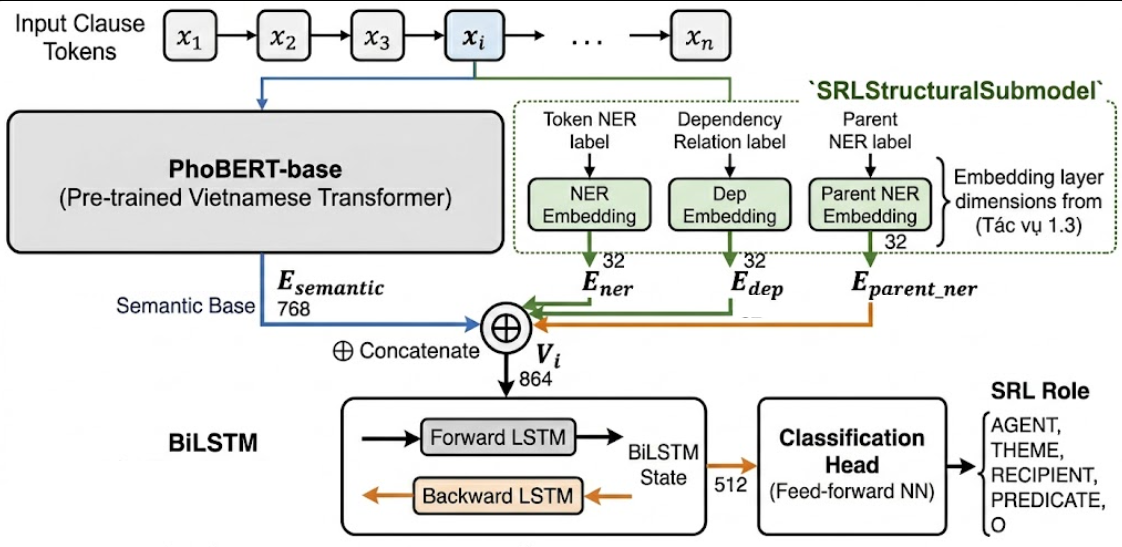
\includegraphics[width=1.0\textwidth]{Image/srl_model.png}
    \caption{Sơ đồ kiến trúc JointSRLModel: Kết hợp Semantic Base, Structural Embeddings và lớp Sequential Modeling.}
    \label{fig:joint_srl_arch}
\end{figure}

Hệ thống vector đầu vào cho mỗi token $x_i$ là một vector tổng hợp $V_i$:
\begin{equation}
V_i = [E_{semantic} \oplus E_{ner} \oplus E_{dep} \oplus E_{parent\_ner}]
\end{equation}

Trong đó:
\begin{enumerate}
    \item \textbf{Semantic Base ($E_{semantic}$)}: Trích xuất từ tầng ẩn cuối cùng của PhoBERT ($768$ chiều). Vector này mang thông tin ngữ cảnh đa chiều, giúp model hiểu nghĩa của từ trong mối tương quan với các từ xung quanh.
    \item \textbf{Structural Embeddings ($E_{ner}, E_{dep}, E_{parent\_ner}$)}: 
    Để tối ưu hóa, hệ thống không đưa các nhãn nhị phân (one-hot) mà thông qua một mạng con \texttt{SRLStructuralSubmodel}. Mạng này ánh xạ các thực thể và quan hệ cú pháp vào một không gian nhúng thấp chiều ($32$ chiều mỗi loại):
    \begin{itemize}
        \item \textbf{Token NER ($E_{ner}$)}: Cung cấp "manh mối" về loại thực thể. Một token là \texttt{PARTY} sẽ có xác suất cao là \texttt{AGENT} (người thực hiện) hoặc \texttt{RECIPIENT} (người thụ hưởng).
        \item \textbf{Dependency Relation ($E_{dep}$)}: Nhãn quan hệ phụ thuộc (như \textit{nsubj, obj, obl}). Ví dụ, một từ có quan hệ \textit{nsubj} với động từ chính gần như chắc chắn đóng vai trò \texttt{AGENT}.
        \item \textbf{Parent NER ($E_{parent\_ner}$)}: Đây là đặc trưng "vượt cấp" độc đáo. Bằng cách nhìn vào nhãn thực thể của từ "cha" (Head word) trong cây cú pháp, model có thể hiểu được phân cấp ngữ nghĩa. Nếu từ cha là một \texttt{PREDICATE} (động từ pháp lý), từ con mang nhãn \texttt{MONEY} sẽ đóng vai trò là \texttt{THEME} (đối tượng giao dịch).
    \end{itemize}
    \item \textbf{Sequential Modeling (BiLSTM)}: 
    Sau khi kết hợp các vector ($768 + 32 \times 3 = 864$ chiều), chuỗi được đưa qua lớp \textbf{BiLSTM} hai chiều với $256$ unit mỗi chiều (tổng $512$). 
    \begin{itemize}
        \item \textit{Forward LSTM}: Nắm bắt thông tin tiền ngữ cảnh.
        \item \textit{Backward LSTM}: Nắm bắt thông tin hậu ngữ cảnh.
    \end{itemize}
    Lớp này đóng vai trò "hòa trộn" giữa tri thức tĩnh (nhãn cấu trúc) và tri thức động (ngữ nghĩa PhoBERT) để đưa ra quyết định cuối cùng về vai trò ngữ nghĩa của token trong dòng chảy của mệnh đề.
\end{enumerate}

\paragraph{Điểm lợi của phương pháp:} 
Việc bổ sung \texttt{Structural Embeddings} đóng vai trò như một cơ chế "Shortcut" (đường tắt). Thay vì bắt PhoBERT phải tự học lại các quy tắc cú pháp phức tạp từ đầu (đòi hỏi dữ liệu cực lớn), chúng ta trực tiếp "tiêm" tri thức ngôn ngữ học vào model. Điều này đặc biệt hiệu quả trong miền dữ liệu hẹp như hợp đồng pháp lý, giúp model đạt độ chính xác cao ngay cả với tập dữ liệu huấn luyện giới hạn.

\paragraph{Mô tả thuật toán xử lý đặc trưng (Inference):}
Hệ thống sử dụng kỹ thuật "Mặt nạ nhãn ký tự" (Character Label Mask) để đảm bảo kết quả trích xuất SRL khớp hoàn toàn với văn bản gốc dù có sự sai lệch giữa tokenizer của Stanza và PhoBERT.

\begin{verbatim}
Algorithm: SRL Character Masking
Input: Predicted SRL labels per token, Original Text, NER Entities
Output: Predicate and Arguments dictionary

1. char_mask = Array of length(Original Text), initialized to None
2. For each entity in NER:
      If entity.label == "PREDICATE":
         Fill char_mask[span] with "PREDICATE"
3. For each token i and its predicted label L:
      Map token i to real_start, real_end in Original Text
      For idx from real_start to real_end:
         If char_mask[idx] is None: char_mask[idx] = L
4. current_role = None, buffer = ""
5. For idx, label in char_mask:
      If label != current_role:
         Flush buffer to results[current_role]
         current_role = label, buffer = char_at(idx)
      Else:
         buffer += char_at(idx)
6. Return results
\end{verbatim}

\paragraph{Ví dụ trực quan:}
\begin{itemize}
    \item \textbf{Mệnh đề}: "Bên A bàn giao vật tư cho bên B."
    \item \textbf{Trích xuất}:
    \begin{itemize}
        \item \texttt{Predicate}: "bàn giao"
        \item \texttt{Agent}: "Bên A"
        \item \texttt{Theme}: "vật tư"
        \item \texttt{Recipient}: "cho bên B"
    \end{itemize}
\end{itemize}

\subsubsection{Phân loại ý định mệnh đề (Task 2.3)}

Tác vụ này xác định chức năng pháp lý của toàn bộ mệnh đề.

\paragraph{Lược đồ ý định (Intents):}
\begin{itemize}
    \item \textbf{Obligation}: Nghĩa vụ bắt buộc thực hiện (từ khóa: "phải", "có trách nhiệm").
    \item \textbf{Prohibition}: Hành vi bị cấm (từ khóa: "không được", "cấm").
    \item \textbf{Right}: Quyền lợi của một bên (từ khóa: "có quyền", "được phép").
    \item \textbf{Termination Condition}: Điều kiện chấm dứt hợp đồng.
    \item \textbf{Other}: Các câu thông tin chung hoặc định nghĩa.
\end{itemize}

\paragraph{Pipeline phân loại đa tầng (Fallback Strategy):}
Vì các hợp đồng pháp lý yêu cầu độ chính xác tuyệt đối, hệ thống được thiết kế theo kiến trúc "phòng ngự nhiều lớp" (Defense-in-depth) thông qua hàm \texttt{classify\_intent} trong tệp \texttt{intent\_classifier.py}. Hệ thống sẽ tuần tự thử nghiệm các mô hình từ độ phức tạp cao đến thấp, đảm bảo luôn có kết quả ngay cả khi gặp lỗi ngoại lệ (exception) hay thiếu hụt tài nguyên (OOM).

\begin{enumerate}
    \item \textbf{Lớp 1 - Robust Transformer (PhoBERT):} Đây là lõi suy luận chính. Cụm văn bản được tách từ (tokenize) bằng thuật toán BPE và đưa vào \texttt{RobustIntentModel}. Nhờ cơ chế Self-Attention, lớp này có khả năng nắm bắt "ý định ngầm" (implicit intent). Ví dụ, câu \textit{"Bên A sẽ thanh toán tiền cọc"} không có từ khóa "nghĩa vụ" rõ ràng, nhưng PhoBERT vẫn phân loại chính xác là \texttt{Obligation} nhờ học được ngữ cảnh khái quát từ hàng ngàn mẫu huấn luyện.
    \item \textbf{Lớp 2 - ML Baseline (TF-IDF + Logistic Regression):} Nếu Lớp 1 thất bại (ví dụ: mô hình chưa được tải vào VRAM), hệ thống sẽ kích hoạt Lớp 2. Tại đây, câu văn được chuyển đổi thành một ma trận thưa (sparse matrix) thông qua \texttt{TfidfVectorizer} với dải n-gram $(1, 2)$. Thuật toán Logistic Regression sau đó sẽ tính toán xác suất $\sigma(W^T \cdot X + b)$ để gán nhãn. Mặc dù không hiểu được thứ tự từ vựng phức tạp, mô hình học máy truyền thống này hoạt động cực kỳ nhanh và nhẹ.
    \item \textbf{Lớp 3 - Rule-based Matching:} Trong kịch bản xấu nhất khi cả hai mô hình AI đều không khả dụng, hệ thống rơi về cơ chế quét từ khóa thuần túy (Heuristic). Thuật toán duyệt qua một từ điển được định nghĩa sẵn (\texttt{INTENT\_KEYWORDS}). Nếu trong câu có chứa cụm "không được phép" hoặc "cấm", nó lập tức trả về \texttt{Prohibition}. Nếu không khớp bất kỳ luật nào, hệ thống gán nhãn an toàn là \texttt{Other}.
\end{enumerate}

\paragraph{Thiết kế Head phân loại và Multi-Sample Dropout:}
Mô hình \texttt{RobustIntentModel} được xây dựng bằng cách kế thừa kiến trúc \texttt{RobertaForSequenceClassification} (nền tảng của PhoBERT) và tích hợp thêm lớp bọc xử lý nhiễu. Điểm cốt lõi của thiết kế này nằm ở việc tối ưu hóa vector đại diện ngữ cảnh (Context Representation) thông qua cơ chế lan truyền song song.

Mặc dù ma trận trạng thái ẩn cuối cùng trả về có kích thước $\mathbf{H} \in \mathbb{R}^{L \times D}$ (với $L$ là độ dài chuỗi, $D=768$), nhưng theo đặc thù của dòng RoBERTa, lớp \texttt{classifier} (\texttt{RobertaClassificationHead}) sẽ thực hiện trích xuất vector tại vị trí token đặc biệt đầu tiên $h_{<s>} \in \mathbb{R}^{D}$. Vector này được coi là "tổng hòa ngữ nghĩa" của toàn bộ mệnh đề nhờ cơ chế Self-Attention.

Để gia tăng khả năng tổng quát hóa trên tập dữ liệu pháp lý nhỏ, lớp bọc \texttt{MultiSampleDropoutWrapper} triển khai kỹ thuật \textbf{Multi-Sample Dropout} \autocite{multidrop}. Thay vì sử dụng một tầng Dropout đơn lẻ, hệ thống tạo ra $K = 5$ nhánh xử lý song song. Thuật toán chi tiết như sau:

\begin{enumerate}
    \item \textbf{Forward Pass:} Vector trạng thái ẩn $\mathbf{H}$ từ PhoBERT được đưa vào module \texttt{MultiSampleDropout}.
    \item \textbf{Parallel Dropout:} Hệ thống áp dụng 5 mặt nạ Dropout khác nhau $M_1, \dots, M_5$ với xác suất loại bỏ ($p$) tăng dần từ $0.1$ đến $0.5$ lên cùng một đầu vào $\mathbf{H}$.
    \item \textbf{Shared Classification:} Cả 5 phiên bản sau Dropout đều được đưa qua cùng một lớp \texttt{classifier} (bao gồm một tầng Dense kết hợp hàm kích hoạt Tanh và tầng Linear cuối cùng).
    \item \textbf{Aggregation:} Logits cuối cùng là trung bình cộng của 5 kết quả đầu ra, giúp triệt tiêu các sai số ngẫu nhiên:
    \begin{equation}
    Z_{final} = \frac{1}{5} \sum_{k=1}^{5} \text{Classifier}(\text{Dropout}_k(\mathbf{H}))
    \end{equation}
\end{enumerate}

Việc áp dụng nhiều mức Dropout khác nhau trong cùng một lần huấn luyện giúp mô hình không bị phụ thuộc quá mức vào bất kỳ nhóm neuron cụ thể nào, từ đó nhận diện ý định pháp lý (như \texttt{Obligation} hay \texttt{Prohibition}) dựa trên các đặc trưng bền vững nhất.

\begin{figure}[H]
    \centering
    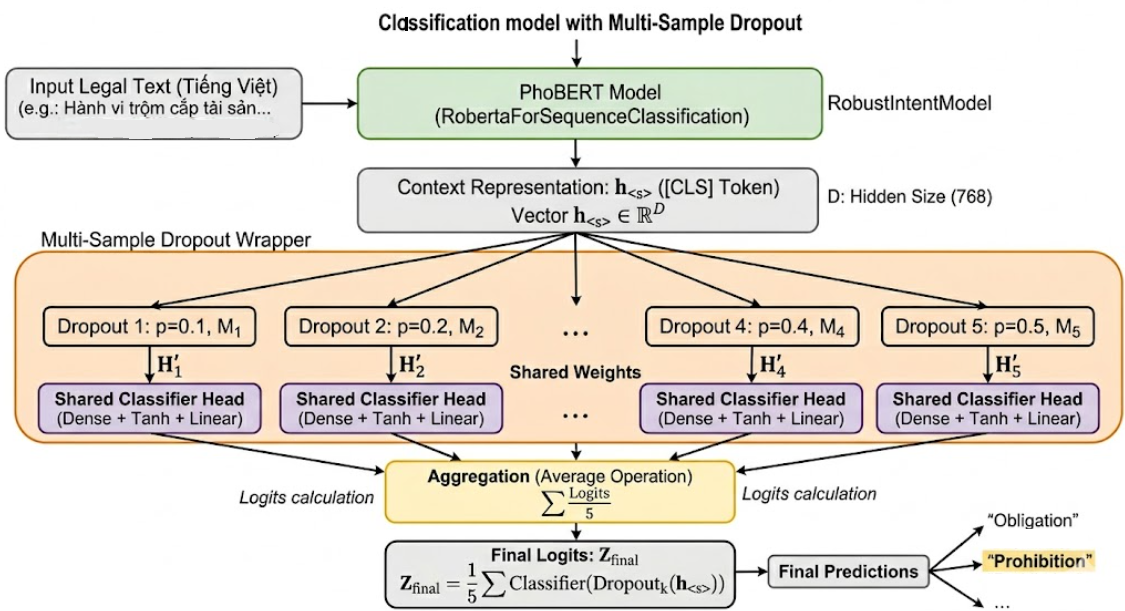
\includegraphics[width=1.0\textwidth]{Image/intent_model.png}
    \caption{Sơ đồ kiến trúc mô hình phân loại với cơ chế Multi-Sample Dropout can thiệp vào Classification Head.}
    \label{fig:intent_arch}
\end{figure}
\pagebreak
\section{Ứng dụng hỏi đáp hợp đồng (Assignment 3)}

Hệ thống hỏi đáp (QA System) trong đồ án này không chỉ đơn thuần là một chatbot RAG (Retrieval-Augmented Generation) cơ bản. Hệ thống được thiết kế theo kiến trúc "Legal Search Architect" - một quy trình truy xuất đa tầng kết hợp giữa hiểu biết ngữ cảnh của LLM và các thông tin cấu trúc (NER, SRL, Intent) đã trích xuất ở Assignment 1 và 2.

\subsection{Kiến trúc hệ thống RAG đa tầng}

Thay vì đưa trực tiếp câu hỏi của người dùng vào cơ sở dữ liệu vector, hệ thống thực hiện một quy trình gồm 3 giai đoạn chính:

\begin{enumerate}
    \item \textbf{Giai đoạn 1 - Lập kế hoạch truy vấn (Search Blueprint):} Sử dụng Gemini để phân tích câu hỏi và tạo ra một "bản thiết kế" tìm kiếm dưới dạng JSON, bao gồm các bộ lọc về thực thể, ý định và vai trò ngữ nghĩa.
    \item \textbf{Giai đoạn 2 - Truy xuất mục tiêu (Targeted Retrieval):} Thực hiện lọc cứng (Hard Filter) trên metadata của ChromaDB và tái xếp hạng (Re-rank) bằng thuật toán chấm điểm SRL Heuristic.
    \item \textbf{Giai đoạn 3 - Sinh câu trả lời có trích dẫn:} Kết hợp ngữ cảnh đã tinh lọc để Gemini tổng hợp câu trả lời cuối cùng theo phong cách văn bản pháp quy.
\end{enumerate}

\begin{figure}[H]
    \centering
    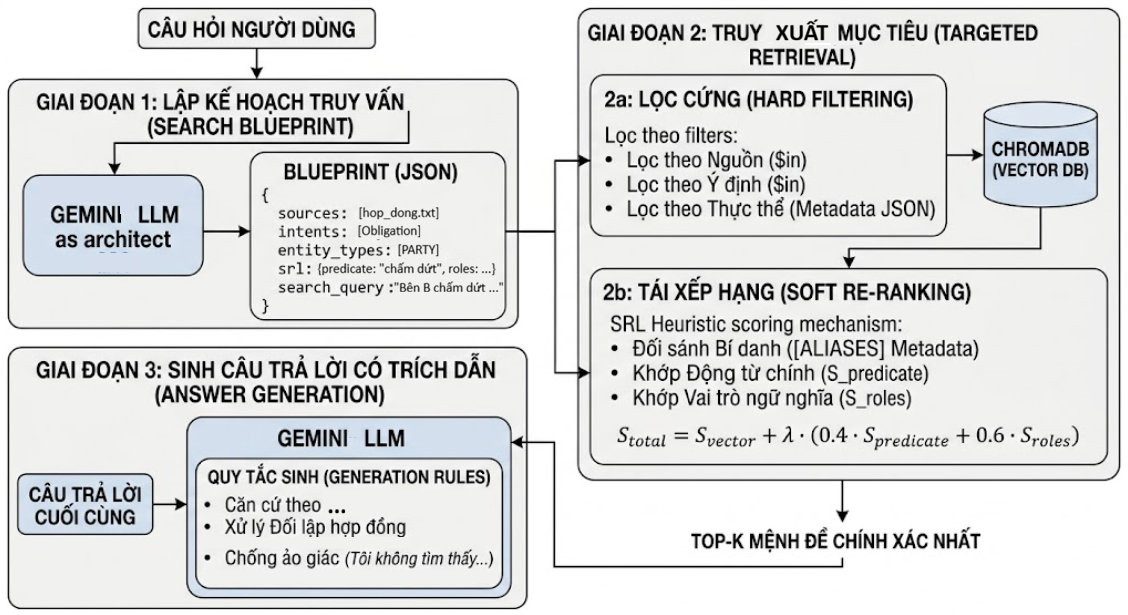
\includegraphics[width=1.0\textwidth]{Image/rag_pipeline.png}
    \caption{Quy trình truy xuất và xử lý của hệ thống QA.}
    \label{fig:rag_flow}
\end{figure}

\subsection{Khối truy xuất tri thức nâng cao (Legal Retriever)}

Đây là thành phần cốt lõi đảm bảo tính chính xác và giảm thiểu hiện tượng "ảo giác". Cơ chế lọc được chia làm hai loại: Lọc cứng (Hard Filter) và Lọc mềm (Soft Re-ranking).

\subsubsection{Cơ chế tạo Search Blueprint bằng Gemini}

Khi nhận câu hỏi, hệ thống gửi một Prompt đặc biệt tới Gemini (xem tại \texttt{src/qa/generator.py}) để yêu cầu mô hình đóng vai trò một kiến trúc sư tìm kiếm. 

\textbf{Ví dụ:} 
\begin{itemize}
    \item \textbf{Câu hỏi:} "Điều gì xảy ra nếu Công ty ABC chậm thanh toán?"
    \item \textbf{Blueprint (JSON) tạo bởi Gemini:}
\end{itemize}

\begin{verbatim}
{
  "sources": ["hop_dong_thue_nha.txt"],
  "intents": ["Termination Condition", "Obligation"],
  "entity_types": ["PARTY", "PENALTY"],
  "srl": {
    "predicate": "thanh toán",
    "roles": {"AGENT": "Công ty ABC", "CONDITION": "chậm"}
  },
  "search_query": "chậm thanh toán xử phạt chấm dứt hợp đồng"
}
\end{verbatim}

\subsubsection{Chiến lược lọc đa tầng (Multi-stage Filtering)}

Dựa trên Blueprint, hàm \texttt{retrieve} trong \texttt{src/qa/ retriever.py} thực hiện lọc theo thứ tự:

\begin{enumerate}
    \item \textbf{Lọc theo Nguồn (Source Filter) và Ý định (Intent Filter):} Đây là bước lọc cứng ngay tại tầng cơ sở dữ liệu vector (ChromaDB) bằng toán tử \texttt{\$in}. Hệ thống chỉ lấy các mệnh đề thuộc đúng file hợp đồng và có ý định pháp lý phù hợp (ví dụ: chỉ tìm trong các câu mang tính "Nghĩa vụ" hoặc "Điều kiện chấm dứt").
    \item \textbf{Lọc theo Thực thể (Entity Filter):} Hệ thống duyệt qua Metadata \texttt{entities} (đã được lưu dưới dạng chuỗi JSON ở bước Ingest, ví dụ: chỉ những mệnh đề chứa loại thực thể như \texttt{PARTY} hoặc \texttt{MONEY} được yêu cầu mới được giữ lại).
\end{enumerate}

\subsubsection{Thuật toán chấm điểm SRL và Tái xếp hạng (Soft Re-ranking)}

Mặc dù Lọc Cứng (Hard Filter) giúp thu hẹp không gian tìm kiếm, độ chính xác của các câu lệnh truy vấn ngữ nghĩa truyền thống (chỉ dựa vào vector embedding) thường bị giảm sút do hiện tượng "tương đồng bề mặt" (surface similarity). Ví dụ, câu hỏi "Ai trả tiền cho Bên A?" và mệnh đề "Bên A trả tiền cho Bên B" có độ tương đồng vector rất cao do trùng lặp từ vựng, nhưng lại mang ý nghĩa trái ngược nhau. 

Để giải quyết vấn đề này, hệ thống áp dụng kỹ thuật \textbf{Tái xếp hạng (Re-ranking) dựa trên Gán nhãn Vai trò Ngữ nghĩa (SRL)}. Hàm \texttt{\_calculate\_srl\_score} (trong \texttt{src/qa/ retriever.py}) đóng vai trò tinh chỉnh điểm số của các ứng viên dựa trên mức độ khớp của từng thành phần cấu trúc (Vị ngữ và các Vai trò).

Thuật toán chấm điểm SRL ($S_{srl}$) được cấu thành từ hai phần chính: Điểm Vị ngữ ($S_{predicate}$) và Điểm Vai trò ($S_{roles}$).

\paragraph{Chấm điểm Vị ngữ ($S_{predicate}$ - Trọng số 0.4):}
Đầu tiên, hệ thống so sánh hành động chính (Predicate) được yêu cầu trong \textit{Search Blueprint} ($P_{query}$) với Vị ngữ đã được trích xuất sẵn trong Metadata của mệnh đề ($P_{doc}$). Các mức độ khớp được xử lý theo quy tắc giảm dần:
\begin{itemize}
    \item \textbf{Khớp tuyệt đối (Exact Match):} Nếu $P_{query}$ hoàn toàn trùng khớp với $P_{doc}$, $S_{predicate}$ đạt tối đa $1.0$ (tương đương $+0.4$ vào tổng điểm).
    \item \textbf{Khớp một phần (Substring Match):} Nếu một từ nằm trong từ còn lại (ví dụ: "thanh toán" và "thanh toán tiền"), hệ thống ghi nhận điểm $0.625$ (tương đương $+0.25$).
    \item \textbf{Khớp ngữ nghĩa (Semantic Embedding Match):} Nếu không có sự trùng lặp từ vựng, hệ thống tính toán Cosine Similarity giữa vector embedding của $P_{query}$ và $P_{doc}$ (sử dụng cùng mô hình \textit{Vietnamese-SBERT}). 
    \begin{equation}
        \text{CosSim}(P_{query}, P_{doc}) = \frac{E_{P_{query}} \cdot E_{P_{doc}}}{\|E_{P_{query}}\| \|E_{P_{doc}}\|}
    \end{equation}
    Nếu $\text{CosSim} > 0.6$, điểm $S_{predicate}$ được tỷ lệ hóa tuyến tính trong khoảng $[0, 0.5]$ (tương đương $+0.2$ vào tổng). Nếu Cosine Similarity thất bại, thuật toán lui về đối sánh mức độ trùng lặp từ vựng (Jaccard Similarity).
\end{itemize}

\paragraph{Cơ chế Đối sánh Bí danh (Alias Matching) cho Vai trò ($S_{roles}$ - Trọng số 0.6):}
Sau khi xác định mức độ khớp của hành động, hệ thống đối chiếu từng vai trò ngữ nghĩa (như \texttt{AGENT}, \texttt{THEME}, \texttt{RECIPIENT}) giữa \textit{Blueprint} và \textit{Metadata} của mệnh đề. Đây là bước quyết định xem "ai làm gì với ai" có thực sự trùng khớp hay không.

Khó khăn lớn nhất trong hợp đồng là tính đa danh xưng. Một thực thể có thể được gọi bằng nhiều cách: "Công ty ABC", "Bên A", hoặc "Bên cho thuê". Nếu chỉ so sánh chuỗi thông thường, "Công ty ABC" và "Bên A" sẽ trả về điểm $0$, dẫn đến việc loại bỏ nhầm mệnh đề quan trọng.

Để khắc phục, hệ thống tận dụng thẻ \texttt{[ALIASES]} được Gemini trích xuất ở khâu tiền xử lý (ví dụ: \texttt{[("Công ty ABC", "Bên A", "Bên cho thuê")]}). Hàm \texttt{\_match\_with\_aliases} thực hiện logic sau cho mỗi vai trò $k$:
\begin{enumerate}
    \item Lấy giá trị yêu cầu $V_{query}^k$ và giá trị trong mệnh đề $V_{doc}^k$.
    \item Nếu $V_{query}^k$ trùng khớp hoàn toàn với $V_{doc}^k$, điểm vai trò $S_{role}^k = 1.0$.
    \item Nếu không, hệ thống tìm nhóm bí danh $G$ chứa $V_{doc}^k$. Nếu tìm thấy, thuật toán duyệt qua toàn bộ các thành viên $a \in G$ để đối chiếu với $V_{query}^k$:
    \begin{itemize}
        \item Nếu $V_{query}^k == a$, điểm $S_{role}^k = 1.0$.
        \item Nếu $V_{query}^k$ nằm trong $a$ (hoặc ngược lại), điểm $S_{role}^k = 0.8$.
        \item Nếu có sự trùng lặp từ vựng (Jaccard), điểm được tính theo tỷ lệ trùng lặp với mức trần là $0.7$.
    \end{itemize}
    \item Nếu $V_{doc}^k$ không thuộc bất kỳ nhóm bí danh nào, thuật toán quay lại tính điểm trùng lặp chuỗi cơ bản với mức trần phạt nặng hơn ($0.6$ cho chuỗi con, và $0.4 \times \text{Jaccard}$).
\end{enumerate}

Tổng điểm vai trò $S_{roles}$ là trung bình cộng điểm của tất cả các vai trò được yêu cầu trong \textit{Blueprint}:
\begin{equation}
    S_{roles} = \frac{1}{N_{roles}} \sum_{k=1}^{N_{roles}} S_{role}^k
\end{equation}

\paragraph{Ví dụ minh họa chi tiết quá trình Re-ranking:}
Giả sử người dùng hỏi: \textit{"Trách nhiệm của Công ty XYZ khi bàn giao vật tư là gì?"}. Hệ thống đang xét một mệnh đề ứng viên ($D_1$) mang metadata: 
\begin{itemize}
    \item \texttt{predicate}: "chịu trách nhiệm"
    \item \texttt{roles}: \texttt{\{"AGENT": "Bên B", "THEME": "kiểm định chất lượng"\}}
    \item \texttt{aliases}: \texttt{[("Công ty XYZ", "Bên B", "Bên nhận thầu")]}
\end{itemize}
Và \textit{Search Blueprint} ($Q$) tạo ra từ câu hỏi yêu cầu:
\begin{itemize}
    \item \texttt{predicate}: "bàn giao"
    \item \texttt{roles}: \texttt{\{"AGENT": "Công ty XYZ"\}}
\end{itemize}

\textbf{Quá trình tính điểm $S_{srl}$ cho $D_1$:}
\begin{enumerate}
    \item \textbf{Vị ngữ ($S_{predicate}$):} $P_{query}$ ("bàn giao") và $P_{doc}$ ("chịu trách nhiệm") không khớp chuỗi. Hệ thống dùng Embedding tính Cosine Similarity. Giả sử kết quả độ tương đồng là $0.3$ (dưới ngưỡng $0.6$). Tính toán Jaccard (không có từ chung) trả về $0.0$. Vậy $S_{predicate} = 0.0$. Đóng góp vào tổng điểm: $0.0 \times 0.4 = \textbf{0.0}$.
    \item \textbf{Vai trò ($S_{roles}$):} Chỉ có vai trò \texttt{AGENT} được yêu cầu trong $Q$. 
    \begin{itemize}
        \item $V_{query}^{AGENT}$ = "Công ty XYZ", $V_{doc}^{AGENT}$ = "Bên B".
        \item Không khớp chuỗi trực tiếp.
        \item Tra cứu Alias: "Bên B" nằm trong nhóm \texttt{("Công ty XYZ", "Bên B", "Bên nhận thầu")}.
        \item Đối chiếu $V_{query}^{AGENT}$ với các thành viên: Thấy "Công ty XYZ" trùng khớp hoàn toàn ($1.0$) với một thành viên trong nhóm.
        \item Suy ra $S_{role}^{AGENT} = 1.0$. Vậy $S_{roles} = 1.0$. Đóng góp vào tổng điểm: $1.0 \times 0.6 = \textbf{0.6}$.
    \end{itemize}
    \item \textbf{Tổng điểm SRL ($S_{srl}$):} $0.0 + 0.6 = \textbf{0.6}$.
\end{enumerate}

Mệnh đề này nhận được điểm SRL khá cao ($0.6/1.0$) dù vị ngữ không hoàn toàn trùng khớp, nhờ hệ thống hiểu rõ "Công ty XYZ" chính là "Bên B" thông qua cơ chế Alias.

\paragraph{Công thức tính điểm tổng hợp ($S_{total}$):}
Cuối cùng, điểm SRL được kết hợp với điểm Vector ban đầu ($S_{vector}$) để tạo ra điểm xếp hạng tổng thể:

\begin{equation}
S_{total} = \min\left( S_{vector} + \lambda \cdot S_{srl} , 1.0 \right)
\end{equation}

Trong hệ thống, $\lambda$ (hệ số điều tiết SRL) được thiết lập mặc định là $0.7$ nhằm cân bằng giữa việc tìm kiếm dựa trên embedding ngữ nghĩa linh hoạt và việc đối sánh cấu trúc ngữ pháp cứng nhắc. Các mệnh đề ứng viên sau đó được sắp xếp giảm dần theo $S_{total}$ và lọc ra Top-K (thường là 10) để đưa vào Context cho LLM sinh câu trả lời.

\subsection{Khối sinh câu trả lời và Trích dẫn}

Sau khi chọn được Top-K mệnh đề có điểm $S_{total}$ cao nhất, hệ thống gửi dữ liệu vào Prompt cuối cùng cho Gemini. 

\subsubsection{Prompt Engineering cho phản hồi pháp lý}
Hệ thống ép buộc Gemini tuân thủ các quy tắc nghiêm ngặt (\texttt{src/qa/generator.py}):
\begin{itemize}
    \item \textbf{Tính căn cứ:} Mọi khẳng định phải bắt đầu bằng cụm từ "Căn cứ theo [Tên hợp đồng] - [Mục/Điều]...".
    \item \textbf{Tính đối lập:} Nếu câu hỏi liên quan đến nhiều hợp đồng, Gemini phải so sánh sự khác biệt giữa các điều khoản của từng bên.
    \item \textbf{Chống ảo giác:} Nếu thông tin không có trong Top-K mệnh đề truyền vào, model bắt buộc phải trả lời "Tôi không tìm thấy thông tin liên quan".
\end{itemize}

\subsubsection{Minh họa kết quả hỏi đáp}

\begin{table}[H]
\centering
\caption{Ví dụ luồng xử lý câu hỏi thực tế}
\begin{tabular}{|p{3cm}|p{10cm}|}
\hline
\textbf{Câu hỏi} & Bên thuê phải trả bao nhiêu tiền mỗi tháng? \\ \hline
\textbf{Truy xuất} & Tìm thấy mệnh đề: "Phí thuê căn hộ được ấn định là 10.000.000 đồng mỗi tháng" trong \texttt{hop\_dong\_thue\_nha.txt}. \\ \hline
\textbf{SRL Score} & Predicate "trả" $\approx$ "ấn định" (0.7); Agent "Bên thuê" $\equiv$ "Bên B" (Alias match 1.0). \\ \hline
\textbf{Câu trả lời} & Căn cứ theo Hợp đồng thuê nhà - Điều III: Phí thuê căn hộ mà Bên thuê (Bên B) phải thanh toán là 10.000.000 đồng mỗi tháng. \\ \hline
\end{tabular}
\end{table}

\subsection{Giao diện người dùng và Tương tác}

Giao diện được triển khai bằng Streamlit (\texttt{ui/app.py}), cho phép người dùng:
\begin{itemize}
    \item Xem trực quan hóa kết quả phân tích từng mệnh đề (NER tags màu vàng, NP chunks màu xanh).
    \item Theo dõi quá trình "suy nghĩ" của hệ thống qua mục \textit{Routing Debug} (hiển thị Blueprint mà Gemini đã lập ra).
    \item Xem chi tiết điểm số (Score Breakdown) của từng nguồn trích dẫn để đảm bảo tính minh bạch.
\end{itemize}
\pagebreak
\section{Thực nghiệm và đánh giá}
\subsection{Thiết lập thực nghiệm}
\subsection{Kết quả đánh giá Mô hình}
\subsection{Đánh giá hệ thống RAG}
\subsection{Phân tích lỗi}

\pagebreak
\section{Kết luận và hướng phát triển}

\subsection{Kết luận}

Đồ án đã hoàn thành mục tiêu xây dựng một hệ thống NLP toàn diện (End-to-End Pipeline) dành riêng cho miền dữ liệu hợp đồng pháp lý tiếng Việt. Những kết quả đạt được bao gồm:
\begin{itemize}
    \item \textbf{Về mặt kỹ thuật:} Triển khai thành công chuỗi xử lý từ tiền xử lý cú pháp (Assignment 1) đến trích xuất ngữ nghĩa chuyên sâu (Assignment 2). Việc sử dụng mô hình PhoBERT kết hợp với kỹ thuật \textit{Multi-Sample Dropout} và \textit{Focal Loss} đã chứng minh được hiệu quả trong việc xử lý các văn bản có độ nhiễu cao và mất cân bằng nhãn đặc thù của ngành luật.
    \item \textbf{Về mặt ứng dụng:} Xây dựng được hệ thống RAG (Assignment 3) với kiến trúc "Legal Search Architect". Điểm sáng của hệ thống là khả năng minh bạch hóa quá trình suy luận thông qua cơ chế Re-ranking dựa trên SRL và Alias Matching, giúp giảm thiểu hiện tượng ảo giác thông tin và cung cấp câu trả lời có tính căn cứ pháp lý cao.
    \item \textbf{Về mặt dữ liệu:} Áp dụng thành công phương pháp \textit{LLM Knowledge Distillation} để tự động tạo tập dữ liệu huấn luyện chất lượng cao từ Gemini Pro, giúp giải quyết bài toán thiếu hụt dữ liệu gán nhãn trong miền hẹp.
\end{itemize}

Hệ thống không chỉ đáp ứng các yêu cầu về mặt học thuật của môn học mà còn có tiềm năng ứng dụng thực tế trong các hệ thống hỗ trợ rà soát hợp đồng tự động (LegalTech).

\subsection{Hạn chế và Hướng cải tiến}

Mặc dù đạt được kết quả khả quan, hệ thống vẫn tồn tại một số hạn chế cần được nghiên cứu cải tiến trong tương lai:

\subsubsection{Cải tiến mô hình Segmentation theo phương pháp Edit-Based}
Hạn chế lớn nhất của mô hình Segmenter hiện tại (Task 1.1) là sử dụng cơ chế gán nhãn thành phần cố định kết hợp với luật tái tổ hợp (\textit{Rule-based Reconstruction}). Phương pháp này gặp khó khăn khi xử lý các câu phức có cấu trúc lồng nhau quá sâu hoặc các câu có biến thể ngữ pháp không nằm trong danh mục các "Type" đã định nghĩa.

\paragraph{Đề xuất phương án Edit-Based Segmentation:}
Thay vì cố gắng gán nhãn và cắt ghép, chúng ta sẽ mô hình hóa bài toán tách mệnh đề thành một chuỗi các thao tác chỉnh sửa văn bản (\textit{Sequence of Edit Operations}). 
\begin{itemize}
    \item \textbf{Cơ chế hoạt động:} Sử dụng kiến trúc Transformer Encoder (như PhoBERT) để dự đoán một tập hợp các hành động (Actions) tại mỗi vị trí token, bao gồm:
    \begin{itemize}
        \item \texttt{KEEP}: Giữ nguyên từ hiện tại.
        \item \texttt{DELETE}: Xóa từ (ví dụ các liên từ "và", "hoặc" dư thừa sau khi tách).
        \item \texttt{SPLIT}: Đánh dấu vị trí ngắt mệnh đề.
        \item \texttt{COPY\_SUBJECT}: Tự động sao chép chủ ngữ của mệnh đề chính vào đầu mệnh đề phụ để đảm bảo tính toàn vẹn ngữ pháp cho câu mới.
    \end{itemize}
    \item \textbf{Ưu điểm:} Phương pháp này cho phép hệ thống "sinh" ra các mệnh đề mới một cách linh hoạt, giữ được mạch văn tự nhiên và không bị bó buộc vào các cấu trúc cố định. Điều này đặc biệt hữu ích cho các câu liệt kê trong hợp đồng nơi chủ ngữ thường bị ẩn đi ở các mục sau.
\end{itemize}

\subsubsection{Tích hợp Đồ thị tri thức pháp lý (Legal Knowledge Graph)}
Hệ thống RAG hiện tại chủ yếu dựa trên tìm kiếm tương đồng vector. Để nâng cao khả năng suy luận logic (ví dụ: xác định mối quan hệ bắc cầu giữa các công ty con trong hợp đồng), hệ thống cần tích hợp thêm \textbf{Knowledge Graph}.
\begin{itemize}
    \item Trích xuất các thực thể và quan hệ (Entity-Relation) từ toàn bộ kho hợp đồng để xây dựng đồ thị.
    \item Sử dụng \textit{GraphRAG} để truy xuất thông tin không chỉ dựa trên văn bản mà còn dựa trên các liên kết logic giữa các điều khoản và thực thể.
\end{itemize}

\subsubsection{Tối ưu hóa tài nguyên và Khả năng chạy Offline}
Hiện tại hệ thống vẫn phụ thuộc vào Gemini API cho các tác vụ khó. Hướng phát triển tiếp theo sẽ là:
\begin{itemize}
    \item \textbf{Quantization:} Nén các mô hình PhoBERT hiện tại (NER, SRL, Intent) sang định dạng \texttt{ONNX} hoặc \texttt{TensorRT} để tăng tốc độ suy diễn trên các thiết bị không có GPU mạnh.
    \item \textbf{Local LLM:} Tinh chỉnh các mô hình ngôn ngữ nhỏ (SLM) như \textit{Vistral-7B} hoặc \textit{Qwen-Legal} để thay thế hoàn toàn API ngoại vi, đảm bảo tính bảo mật tuyệt đối cho dữ liệu hợp đồng của khách hàng.
\end{itemize}
\pagebreak
\nocite{*}
\printbibliography[heading=bibintoc]
\end{document}
